\documentclass[11pt,letter]{article}
\usepackage{etex}
\usepackage[top=0.65in,bottom=0.9in,left=0.85in,right=0.85in]{geometry}

%\def\baselinestretch{1.25}
\def\baselinestretch{1.0}

\usepackage[greek, english]{babel}
%\usepackage{multicol}
\usepackage[thinlines]{easytable}

%\usepackage[draft]{graphicx}
\usepackage{graphicx}
\usepackage[export]{adjustbox}

\usepackage{caption}
\usepackage{subcaption}

\usepackage{setspace}

% The use of the times package forces the use of the type-1 times
% roman font, but the times roman font does not look nice.
% Besides the times roman font still does not print correctly on
% the dopy printer.
%\usepackage{times}


\usepackage{fancyhdr}
\usepackage{amsmath}
\usepackage{amssymb}
\usepackage{bm}
\usepackage{bbold}
\usepackage{parskip}

\newcommand{\kb}{\ensuremath{k_{\text{B}}}}

\newcommand{\bv}[1]{\ensuremath{\bm{#1}}}
\newcommand{\Lc}{\ensuremath{L_{\mathrm{c}}}}
\newcommand{\dsig}[1]{\ensuremath{ \frac{ d\,\sigma_{#1} }{d\,\Omega} }}

\newcommand{\isat}{\ensuremath{I_{\mathrm{sat}}}}
\newcommand{\iisat}{\ensuremath{I_{\mathrm{p}}/I_{\mathrm{sat}}}}
\newcommand{\Iqtof}{\ensuremath{I_{\bv{Q}\infty} }}
\newcommand{\Itof}[1]{\ensuremath{I_{\bv{#1}\infty} }}
\newcommand{\Iq}{\ensuremath{I_{\bv{Q}} }}
\newcommand{\iq}{\ensuremath{i_{\bv{Q}} }}
\newcommand{\Iqma}{\ensuremath{I_{\bv{Q}_{\text{MA}}} }}
\newcommand{\Ima}[1]{\ensuremath{I_{\bv{#1}_{\text{MA}}} }}
\newcommand{\iqma}{\ensuremath{i_{\bv{Q}_{\text{MA}}} }}
\newcommand{\jqma}{\ensuremath{j_{\bv{Q}_{\text{MA}}} }}
\newcommand{\Iqmatof}{\ensuremath{I_{\bv{Q}_{\text{MA}\infty}} }}
\newcommand{\is}{\ensuremath{i_{S}} }
\newcommand{\iqT}{\ensuremath{i_{\bv{Q}_{T}} }}
\newcommand{\ipith}{\ensuremath{i_{\bv{\pi}/\bv{\theta}}}}
\newcommand{\fpith}{\ensuremath{f_{\bv{\pi}/\bv{\theta}}}}
\newcommand{\iT}[1]{\ensuremath{i_{\bv{#1}_{T}} }}
\newcommand{\ima}[1]{\ensuremath{i_{\bv{#1}_{\text{MA}}} }}
\newcommand{\fma}[1]{\ensuremath{f_{\bv{#1}_{\text{MA}}} }}
\newcommand{\jma}[1]{\ensuremath{j_{\bv{#1}_{\text{MA}}} }}

\newcommand{\pin}{\ensuremath{ P_{\text{i}}} }
\newcommand{\pret}{\ensuremath{ P_{\text{r}}} }
\newcommand{\win}{\ensuremath{ w_{\text{in}}} }
\newcommand{\wret}{\ensuremath{ w_{\text{r}}} }
\newcommand{\wir}{\ensuremath{ w_{\text{ir}}} }

\newcommand{\pgr}{\ensuremath{ P_{\text{gr}}} }
\newcommand{\wgr}{\ensuremath{ w_{\text{gr}}} }

\newcommand{\dbl}{\ensuremath{ \uparrow\! \downarrow \, }}
\newcommand{\spup}{\ensuremath{ \uparrow }}
\newcommand{\spdn}{\ensuremath{ \downarrow}}

\newcommand{\rdiag}{\ensuremath{ r_{\text{d}} } } 

\begin{document}

\section{ Compensated optical lattice} 

Our experiments take place in a compensated simple cubic optical lattice
potential, which is formed at the intersection of three orthogonal axes, see
Fig.~\ref{fig:compensated_lattice_simple_schematic}.  Along each axes, a 1D
lattice potential is formed by retro-reflecting a red-detuned Gaussian beam,
which results in a sinusoidal intensity pattern along the beam.  Overlapped onto
each of the lattice beams we have a compensation beam, which is blue-detuned
and thus produces a repulsive potential.   The compensation beam is not
retro-reflected, so it does not form a standing wave potential, see
Fig.~\ref{fig:compensated_lattice_simple_schematic}.  
\begin{figure}
    \centering
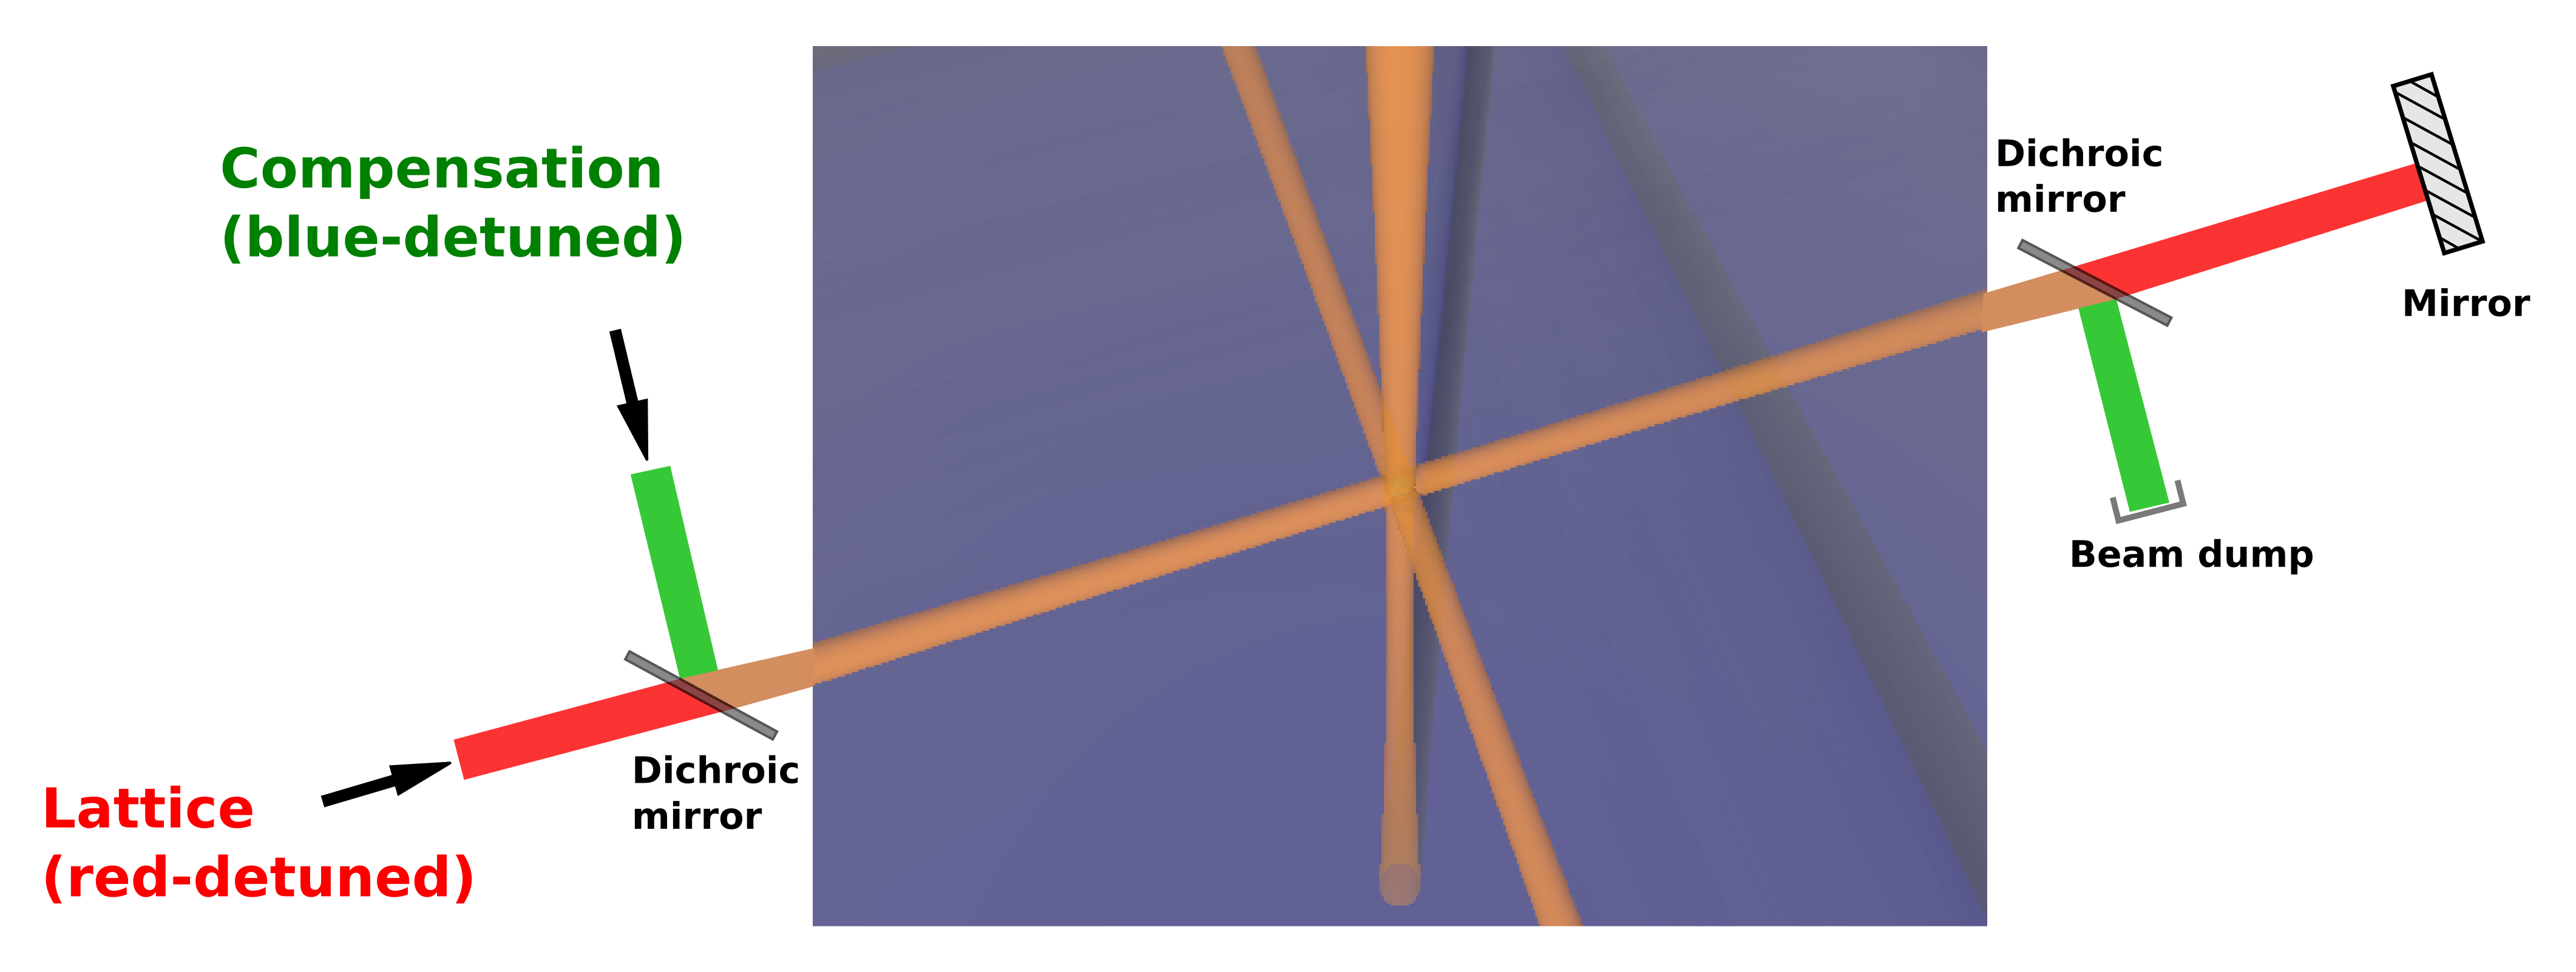
\includegraphics[width=0.8\textwidth]{figures/compensated_lattice_simple_schematic.png}
\caption{Simplified schematic of the compensated lattice
setup}\label{fig:compensated_lattice_simple_schematic}
\end{figure}

The lattice beam that propagates along the $x$ axis produces a potential of the
form 
\begin{equation}
 \frac{ V_{L}( x; y,z) }{E_{R}} = 
  - s_{0} \exp\left[- 2 \frac{ y^{2} + z^{2} }{w_{L}^{2}} \right]
  \cos^{2}( k_{L} x ) 
\end{equation}
where $s_{0}$ is the lattice depth at the center of the potential,  $w_{L}$ is
the lattice beam waist and $k_{L} = 2\pi/\lambda_{L}$ is the wavenumber of the
lattice light.
The compensation beam that propagates along $x$ produces a potential  
\begin{equation}
 \frac{ V_{C}( x; y, z) }{E_{R}} = 
   g_{0}  \exp\left[ -2 \frac{ y^{2} + z^{2} }{w_{C}^{2}} \right] 
\label{eq:Vcomp}
\end{equation}
where  $g_{0}$ is the depth (or rather height since it is repulsive) of the
compensating potential, and $w_{C}$ is the beam waist of the compensation
beam\footnote{We will use the letter $s$ for the lattice depth and the letter
$g$ for the compensation depth.  Both $s$ and $g$ are taken to be in units of
the recoil energy of a lattice photon, $E_{R}$.  To facilitate dimensional
verification of the expressions we will explicitly indicate when a quantity is
obtained in units of $E_{R}$.  Note that $s$ and $g$ are taken always to be
positive numbers.  }.

The combined potential of lattice plus compensation for the beams propagating
along $x$ is 
\begin{equation}
  V_{1D}( x; y ,z ) = V_{L}(x; y,z) + V_{C}(x; y, z)
\end{equation}

The total potential for our simple cubic lattice is given by 
\begin{equation}
  V_{3D}(x, y, z)  =  V_{1D}( x; y,z) + V_{1D}( y; z,x) + V_{1D}(z; x,y)
\end{equation}


In what follows we will study the properties of a two spin-state mixture of
fermionic atoms in the compensated optical lattice potential.   We are
interested in the total entropy capacity of the potential, and also on the
possibility of evaporative cooling in the lattice potential.   

We will use the high-temperature series expansion (HTSE),  an analytical
solution to the Hubbard model that is valid at high-temperatures\footnote{ The
HTSE is very good for $T \gg t$ and works down to $T/t \sim 1.8$ }.  This
solution gives us the thermodynamic quantities (density, double occupancy,
entropy per particle, etc.)  for a homogeneous system;  we then use the local
density approximation (LDA) to explore the properties of the sample in the
compensated lattice potential.  

\section{General aspects of the potential }

Before we go ahead and deploy the full machinery of the LDA we will discuss
some general aspects of the potential. 

One of the important things to note is that at each point in space  we will, in
general, have three different lattice depths, associated with each of the
$x,y,$ and $z$ lattice directions.  For this reason the potential is difficult
to visualize.  To make thinks simpler, we can plot trap profiles along the 111
direction.   Along this direction we have that the lattice depth is the same in
all three directions\footnote{We will use the notation $\rdiag$ to represent
the distance along the 111 diagonal line.}:
\begin{equation} 
  s_{x}( \rdiag ) = s_{y}( \rdiag ) = s_{z}( \rdiag ) = 
  s_{0} \exp \left[ - \frac{ 4 \rdiag^{2} }{3 w_{L}^{2} } \right]  
  \equiv s(\rdiag) 
\end{equation}

The bottom envelope of the lattice potential is given by 
\begin{equation}
  \frac{ V_{L,\text{env}}( \rdiag ) }{E_{R}} = -3 s_{0} 
  \exp \left[ - \frac{ 4 \rdiag^{2} }{3 w_{L}^{2} } \right]  
\end{equation} 


An important aspect of a lattice potential is that the avaliable energy levels
exhibit a band structure.  The lowest energy of the band, $E_{0}$, measured
from the potential envelope $V_{L,\text{env}}$, is given by the zero-point
energy of the 3D harmonic oscillator centered at the bottom of each lattice
site.   This harmonic oscillator result is only valid for deep lattices
($\gtrsim 10\,E_{R}$) but we will use it here for illustrative purposes: 
\begin{equation}
  \frac{E_{0}}{E_{R}} = 
     \frac{ \frac{3}{2} \hbar \omega_{0} }{ E_{R} } = 3\sqrt{ s } 
\end{equation} 
We can also obtain an expression for the bandwidth $W$, valid in the limit of
deep lattices~\cite{Bloch2008}:
\begin{equation}
  \frac{W}{E_{R}} =  
  \frac{12 t}{E_{R} }  = \frac{48}{\sqrt{\pi}} s^{3/4} e^{-2\sqrt{s}} 
\end{equation}

The energy of the first excited band in the lattice corresponds to an
excitation along one of the lattice directions, which adds an extra $\hbar
\omega_{0}$  to the bottom of the band.  In Fig.~\ref{fig:lattice_general} we
have plotted the lattice potential envelopes along with the envelopes of the
lowest band and a line that is representative of the energy levels of the first
excited band.  
\begin{figure}
    \centering
    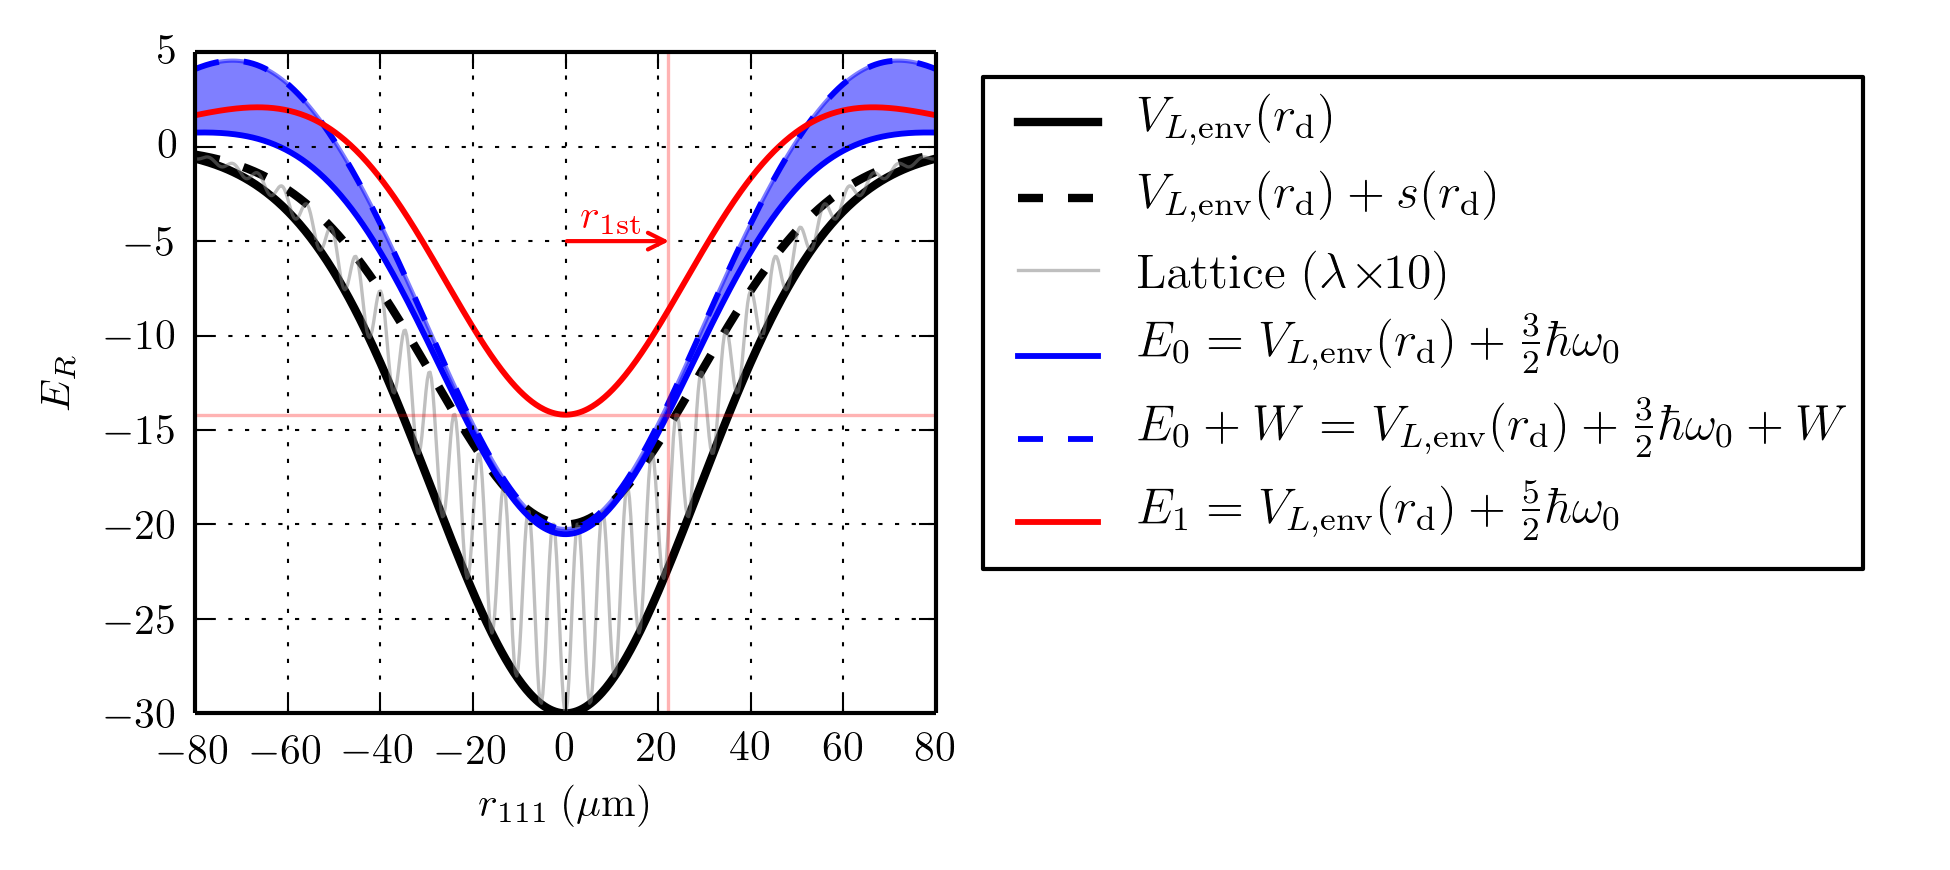
\includegraphics[width=0.8\textwidth]{figures/lattice_general.png}
    \caption{Diagonal profiles for a 10$E_{R}$ lattice with $w_{L}=47\,\mu$m. }
\label{fig:lattice_general}
\end{figure}

Also indicated in Fig.~\ref{fig:lattice_general} is the radius, $r_{1}$, at
which the energy of the lowest band is equal to band gap at the origin:
\begin{equation}
  E_{0}(\rdiag = r_{1} ) -  E_{0}( \rdiag=0)  = 
  E_{1}(\rdiag = 0 ) -  E_{0}(\rdiag=0) 
\end{equation} 
 In order to stay well within the single band approximation of the Hubbard
model, our sample needs to have a size that is much smaller than $r_{1}$. 

\subsection{Lattice locking}

On occasion we will raise the lattice depth suddenly, in order to freeze out any
further tunneling.   This will be useful to get the maximum possible
Debye-Waller factor when performing a Bragg scattering measurement,  or it will
also be useful to keep the density distribution frozen when sweeping across the
narrow Feshbach resonance to make doublons.   

For Feshbach sweeps across the narrow resonance we have found that going
across from 80\,$a_{0}$ to 61\,$a_{0}$ in 24 ms gives us nearly 100\%
conversion efficiency. For some measurements we blow away any remaining atoms
with a resonant light pulse and sweep back across the resonance to dissociate
the molecules.  For such a procedure we require the density distribution to
remain locked for times up to 48~ms.  To have less than 0.1 tunneling events
in 48~ms, the tunneling rate in the lattice should be less than 2~Hz. 

On Fig.~\ref{fig:lattice_lock} we show the tunneling rate as a function of
lattice depth, and we see that to achieve 2~Hz one needs $\approx 44\,E_{R}$.
With that in mind we have to consider that as we lock-up the lattice to
$44\,E_{R}$ we want to stay within the single band Hubbard model.
Figure~\ref{fig:lattice_lock} also shows the atom number, $N_{1}$,
corresponding to a sample with density $n=1$ atom per site sample filled up to
$r_{1}$. For atom numbers equal or greater than $N_{1}$ the single band
approximation breaks down.   
\begin{figure}
        \centering
        \begin{subfigure}[t]{0.48\textwidth}
		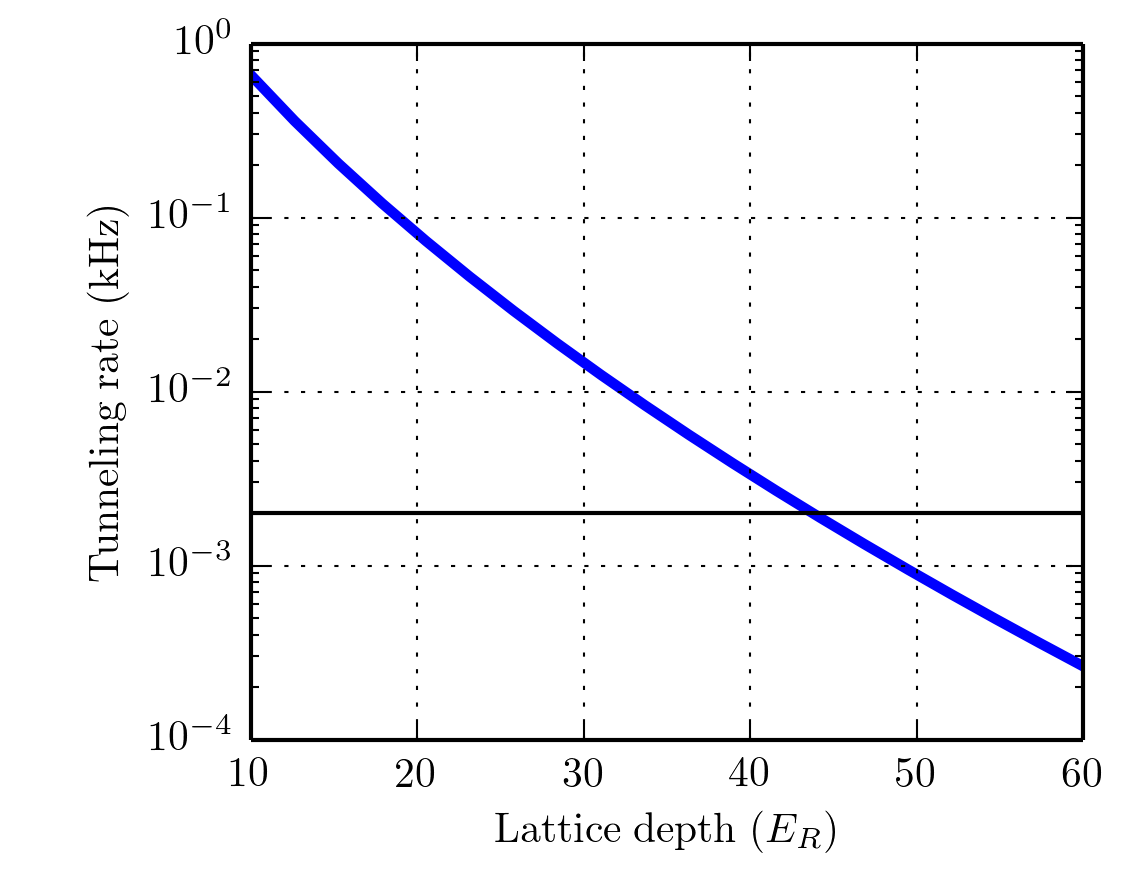
\includegraphics[width=\textwidth]{figures/lattice_tunneling.png}
\caption{Tunneling rate.  The black line is at 2~Hz, which is the rate required
to keep the lattice frozen during a measurement of the double occupancy.}
                \label{fig:lattice_lockA}
        \end{subfigure}
        ~ %add desired spacing between images, e. g. ~, \quad, \qquad etc.
          %(or a blank line to force the subfigure onto a new line)
        \begin{subfigure}[t]{0.48\textwidth}
		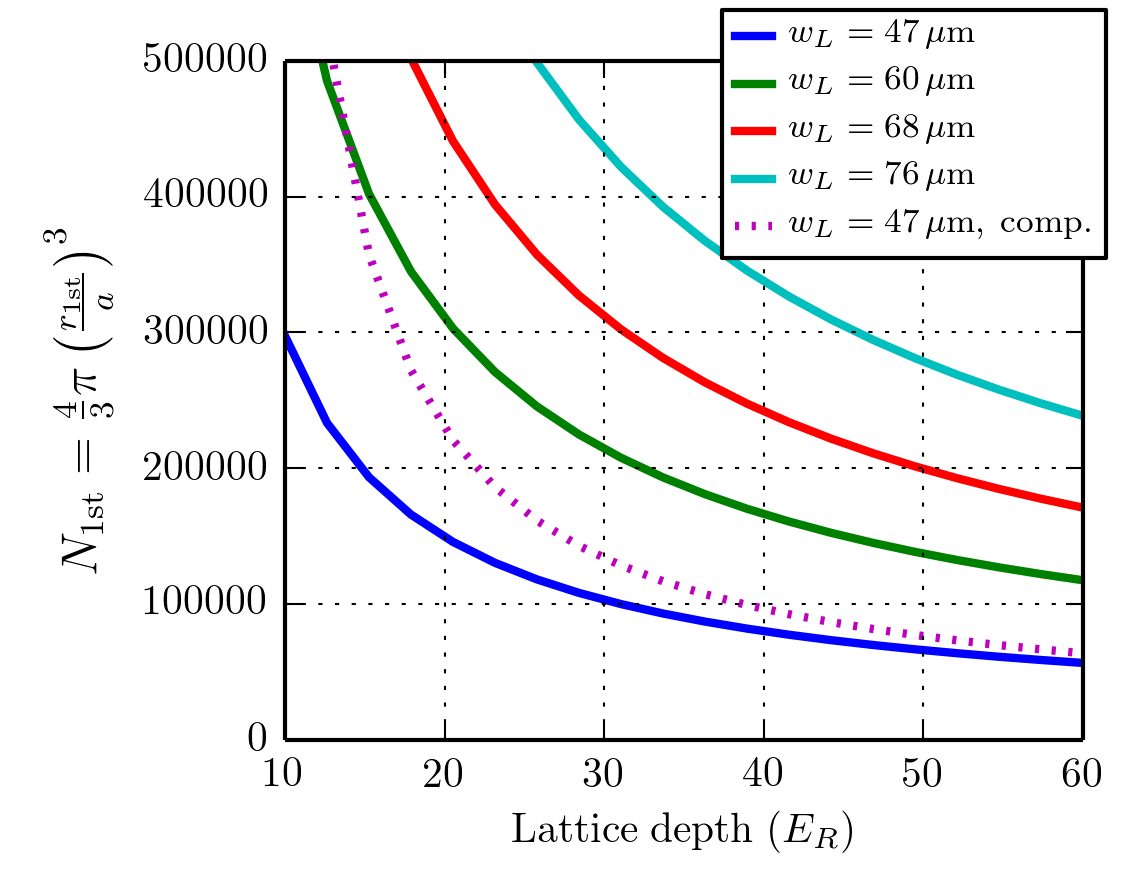
\includegraphics[width=\textwidth]{figures/lattice_lock.png}
\caption{Maximum atom number to stay in the single band regime.  The dashed
line includes 3\,$E_{R}$ of compensation, with a compensation beam waist of
$w_{C}=40\,\mu$m.}
                \label{fig:lattice_lockB}
	\end{subfigure}%
	\caption{Considerations to be taken when locking the lattice to freeze
out tunneling.}\label{fig:lattice_lock}
\end{figure}

From Fig.~\ref{fig:lattice_lock} we see that for samples of $N=300,000$ atoms
and a lattice beam waist of $47\,\mu$m,  the maximum lock depth to stay in the
single band regime is $\approx 10\,E_{R}$.   Currently, when doing Bragg
scattering measurements, we lock the lattice up to 20\,$E_{R}$ to get the
largest possible Debye-Waller factor.   In the Bragg experiment we use a
compensation of 3\,$E_{R}$ to flatten out a 7,$E_{R}$ lattice and we leave it
on during the lattice lock.   Having the $3\,E_{R}$ of compensation gives us a
maximum atom number of $\approx$230,000 atoms to stay in the single band
regime, as is shown with the dotted line in Fig.~\ref{fig:lattice_lock}.

Unfortunately, we have found that Feshbach molecules scatter green light
strongly.  If we have any green light on we loose them in just a few
milliseconds.  This means that, when considering doublon measurements, we
cannot afford to have any green compensation light on.  

With this in mind we see from Fig.~\ref{fig:lattice_lock} that, in order to be
able to lock the lattice up to $44\,E_{R}$  and have the capacity to hold
$N\approx 250,000$ in the single band regime, we would require a lattice beam
waist as large as $70\,\mu$m. 


\subsection{Characteristic energy}

In the previous subsection we considered the number of atoms required to fill
up a sample (at zero temperature and  a density of one per site) up to a
certain radius.    For a given number of atoms and a band shape,  that band
energy at that radius is (up to some constants that will be specified below)
referred to as the characteristic energy of the trap, $E_{\text{t}}$. 


%%Since the band is curved, as shown in
%%Fig.~\ref{fig:lattice_general}, for a given radius there is an associated
%%energy of the band.  
%%
%% The exact shape of the potential and the number of atoms
%%define this energy, which is referred to as the characteristic energy of the
%%trap, $E_{t}$.  
%%
%%We will give the exact definition of $E_{t}$ in the paragraphs
%%below.  
 
%Traditional lattice setups use large lattice beam waists, so the bandwidth,
%$W$,  is nearly constant as a function of position in the trap.  For a
%reasonable number of atoms ($<$1 million), if the lattice beam waist is large,

For a sample of atoms with radius small compared to the lattice beam waists
we can do a series expansion of the  potential envelope and the band bottom to
obtain
\begin{equation}
\begin{split}
    \frac{ V_{L,\text{env}}( \rdiag ) }{ E_{R} }  & =   
        -3 s_{0}  + \frac{ 4 s_{0} }{w_{L}^{2}} \rdiag^{2}  \\
    \frac{ \frac{3}{2}\hbar \omega_{0} }{ E_{R} } & = 
        3 \sqrt{ s_{0}} - \frac{ 2 \sqrt{s_{0}}}{w_{L}^{2}} \rdiag^{2} 
\end{split}
\label{eq:lattice-expand-harmonic}
\end{equation}

The harmonic approximation to the lowest band in the lattice is then 
\begin{equation} 
   \frac{ E_{0}(\rdiag) }{E_{R} }  = 
       \left(\frac{ 4 s_{0} - 2 \sqrt{ s_{0} } }{ w_{L}^{2} } \right)\rdiag^{2} 
       \equiv  \alpha_{\text{t}}  \left( \frac{ \rdiag}{a} \right)^{2}
\end{equation}
where $a=\lambda/2$ is the lattice spacing.  This defines $\alpha_{\text{t}}$
as 
\begin{equation}
 \alpha_{\text{t}} =  \frac{ 4s_{0} - 2\sqrt{s_{0}}}{ (w_{L}/a)^{2} } 
\end{equation}
The characteristic energy of the trap is defined as
\begin{equation} 
  \frac{ E_{\text{t}} }{E_{R}} =  \alpha_{\text{t}} \left(  \frac{ 3N }{ 4\pi }
\right)^{2/3}
\label{eq:characteristic-energy} 
\end{equation}
where $N$ is the total atom number.  It is seen here that the characteristic
energy is the energy of the lowest band at a radius given by 
\begin{equation}
  \frac{ \rdiag }{ a } =  \left( \frac{ 3N }{ 4 \pi} \right)^{1/3}
  \ \ \Rightarrow   \ \ 
  N = \frac{1}{d^{3}} \left(   \frac{4}{3} \pi \rdiag^{3}  \right)
\end{equation}
This radius is simply the size occupied by the $N$ atoms at a density of one
atom per site.  

 
\textbf{Note:} Usually the characteristic energy is defined using the radius of
the sample at a density of two atoms per site~\cite{Schneider2010}.  Perhaps
this is good if one wants to assess the formation of a band insulator with
respect to the band gap.   When dealing with Mott insulating states and
comparing $E_{t}$ with the Mott gap, $U$, a density of one atom per site on the
definition is the best choice, and the one we adopt here.  


The characteristic energy is a useful quantity because it provides a
length-scale-free way of assessing  the level of confinement in the
trap\footnote{ As an alternative measure of the same concept, the
characteristic filling is defined as~\cite{Jordens2010}.
\begin{equation} 
    \rho_{\text{t}} = N \left( \frac{ \alpha_{t} }{ 6 t } \right)^{3/2}
    =  \frac{8\pi}{3} \left( \frac{ E_{\text{t}} }{ 6 t}   \right)^{3/2}  
\end{equation}
Using the characteristic filling it is a little bit more cumbersome to quickly
get an idea of the length-scale-free filling as one has to convert the
interaction energy to an effective density in order to make a well informed
comparison.   It is always easier to just compare $U$ to $E_{t}$. }.
Regardless of the waist of the lattice beams, for a given interaction strength
$U$, a Mott-insulating core  at the center of the sample  can be achieved if
$E_{\text{t}} \approx U/2 $.   Notice that such a characteristic energy
can be achieved experimentally in either of two ways: changing the confinement,
$\alpha_{\text{t}}$, or changing the atom number, $N$.  


To give an example of the use of the characteristic energy, we consider our
current setup with a beam waist $w_{L}=47\,\mu$m.   In a 7\,$E_{R}$ lattice
(without compensation)
\begin{equation}
\begin{split}
  \alpha_{\text{t}} & =  2.909 \times 10^{-3} \\
   t & = 4.88 \times 10^{-2}\,E_{R}  \\ 
\end{split}
\end{equation}
With an interaction strength $U/t = 24$, the atom number required to make an
insulating state with $n=1$ at the center is 
\begin{equation} 	
 N = \frac{4\pi}{3}  
    \left(  \frac{ U/E_{R} }{ 2 \alpha_{\text{t}} } \right)^{3/2}  
     \approx 12,000 \ \text{atoms}  
\end{equation}
We will see in a later section that this estimate agrees with the full
machinery of the LDA.  

In actual experiments typically the main constraint is the atom number.  The
shape and depth of the traps can be adjusted around the achievable atom number
such that one can access the phases of interest.  In our case these are
the Mott insulator state and the antiferromagnetic Mott-insulator
which both require a density of one atom per site at the center.  


A plot of $E_{\text{t}}/t$ as a function of lattice beam waist for a fixed atom
number, $N$=500,000 is shown in Fig.~\ref{fig:Et-waist}.   We use a black line
to denote the value of $U/2t$ for a scattering legth of 650$a_{0}$ in a
10\,$E_{R}$ lattice.  We see that achieving half-filling with the confinement
provided only by the red-detuned lattice requires a lattice beam waist of
$\approx 160\,\mu$m.  
\begin{figure}
    \centering 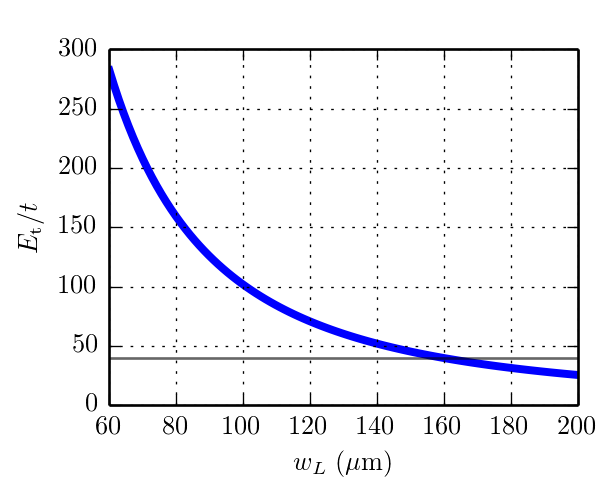
\includegraphics[width=0.5\textwidth]{figures/Et-waist.png}
\caption{Characteristic energy as a function of beam waist for $N=500,000$
atoms. The black line denotes $U/2t$,  which should be the
characteristic energy required to obtain a half-filled sample at the center of
the potential.}
\label{fig:Et-waist}
\end{figure}
In the next section we will see how the addition of the compensating potential
can help us achieve a Mott insulating state using a smaller waist lattice for
the lattice beams.


\subsection{Compensation}

As we have stated, we are interested in exploring the idea of evaporative
cooling in a lattice and also the concept of the entropy capacity of the
lattice system.  We will see that for both these two ideas it will be necessary
to introduce the concept of compensation.  Compensation is a way of reducing
$\alpha_{\text{t}}$ for a given lattice beam waist, such that large system
sizes can be achieved on a smaller beam waist lattice.  

For cooling it is necessary to   have the boundary of the potential as close as
possible to the edge of the sample and compensation helps achieve that.   For
entropy redistribution in the sample, one may gain advantage from the
inhomogeneity in the Hubbard parameters that arises from small lattice beam
waists.  

With the addition of repulsive compensation beams with depth $g_{0}$ and beam
waist $w_{C}$,  as in Eq.~\ref{eq:Vcomp},  we can expand the lowest band of the
lattice in a power series as  
\begin{equation}
\begin{split} 
  \frac{E_{0}(\rdiag)}{E_{R}}  & \approx   
  3( g_{0} + \sqrt{s_{0}} - s_{0} ) 
  + \left[ 
    \frac{ 4s_{0} - 2\sqrt{s_{0}} }{w_{L}^{2} } 
   - 
  \frac{ 4 g_{0} }{ w_{C}^{2}} \right]
  \rdiag^{2} 
  +  \left[  \frac{ - 8 s_{0} + 2\sqrt{s_{0}} }{3 w_{L}^{4} } + 
    \frac{ 8 g_{0} }{3 w_{C}^{4} }  \right] \rdiag^{4}   \\
 &  \equiv  ( A_{0} + A_{2} \rdiag^{2} + A_{4} \rdiag^{4}  ) / E_{R}
\end{split}
\end{equation}

\paragraph{Enlarging the Mott plateau} We define  the beam waist ratio $\alpha
= w_{L}/w_{C}$ as in~\cite{Mathy2012}.  We see that we can completely cancel
the quadratic term of the confinement by choosing 
\begin{equation}
 g_{0} = \frac{  4 s_{0} - 2 \sqrt{s_{0}} }{ 4 \alpha^{2} }  
  \equiv g_{\text{quartic}} 
\end{equation}
This choice of $g_{0}$ will be the most favorable in enlarging the size of the
$n=1$ region of the cloud because it will provide a band that is flat at the
center.  We point out that, for $\alpha > 1$,  if we use a compensation larger
than $g_{\text{quartic}}$, the band profile would have a bump in the center.
We have observed epxerimentally that in that case it becomes hard to align the
compensation beams such that the sample actually stays at the center of the
trap.

In our current experiments we use $s_{0}$=7 and our beam waists are
approximately $w_{L}=47\,\mu$m and $w_{C}=40\,\mu$m, which gives
$\alpha=1.175$.  The necessary compensation to flatten the band would be
$g_{\text{quartic}} =  4.11 $




\paragraph{Evaporation.} We want to consider the possibility of evaporative
cooling in a sample that has $n=1$ at the center.  Half-filling implies that
athe radius of the cloud is $r_{\text{hf}}$, such that 
\begin{equation} 
  E_{0}(\rdiag = r_{\text{hf}} ) -  E_{0}( \rdiag=0 ) =  U/2
  \label{eq:half-filling-radius} 
\end{equation}  
In order to maximize the evaporation rate for a half filled sample we need
$E_{0}(r_{\text{hf}})$ to come as close as possible to the evaporation
threshold, which in our system is the energy required to escape along one of
the lattice beams: 
\begin{equation} 
  E_{\text{th}} = ( g_{0} + \sqrt{s_{0}} - s_{0} ) E_{R} 
\end{equation}

The best we can do is set  $E_{\text{th}}= E_{0}(r_{\text{hf}}) $ which
results in
\begin{equation}
  -2( g_{0} + \sqrt{s_{0}} - s_{0} ) E_{R} = U/2  
\end{equation}  
To maximize the size of the Mott plateau we set $g_{0} = g_{\text{quartic}}$,
and then we solve for the beam waist ratio $\alpha_{\text{evap}}$, which
optimizes the evaporation rate in the lattice. 
\begin{equation}
 \alpha_{\text{evap}}^{2} =  \frac{ 4 s_{0} - 2 \sqrt{s_{0} }}
    { 4s_{0} - 4 \sqrt{s_{0}}  - U/E_{R} }  
\end{equation} 
 
For a deep lattice ($\gtrsim 10\,E_{R}$) the \textbf{on-site interactions}
can be expressed analytically as 
\begin{equation}
  \frac{U}{E_{R}}  =  4 \sqrt{2\pi} \frac{ a_{s} }{\lambda}  s^{3/4} 
  \label{eq:onsite-analytic}
\end{equation} 
The scattering length is usually expressed in units of the Bohr radius,
$a_{0}$, so it is useful to keep in mind that for our 1064~nm lattice
$\lambda = 20113 a_{0}$.  In our experiment we want to avoid very large
scattering lengths because they give rise to fast inelastic losses that scale
as $a_{s}^{4}$.   Reasonable values are up to 800\,$a_{0}$.   In a 7\,$E_{R}$
lattice a scattering length $a_{s}=800\,a_{0}$ implies an interaction
strength $U/t=30$.   In Fig.~\ref{fig:alpha-evap-optimal} we show plots of
$\alpha_{\text{evap}}$ for various values of $U/t$.   
\begin{figure}
    \centering
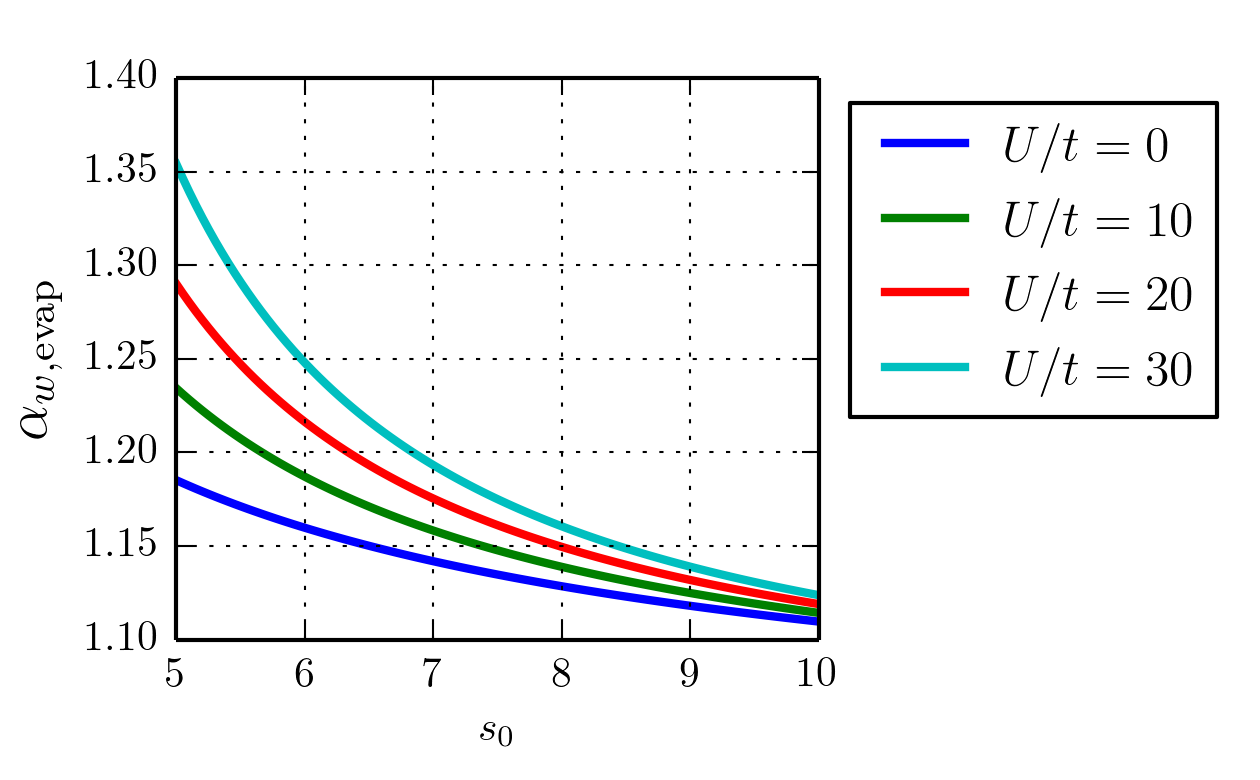
\includegraphics[width=0.5\textwidth]{figures/alpha-evap-optimal.png}
\caption{Optimal beam waist ratio for enlarging the central flat portion on
the band and maximizing the rate of evaporative cooling. }
\label{fig:alpha-evap-optimal}
\end{figure}

We can see that for a 7\,$E_{R}$ lattice $\alpha_{\text{evap}}$ is
between 1.15 and 1.20.  This beam waist ratio is obtained for
$g_{0}=g_{\text{quartic}}$ so the size of the Mott plateau is maximized, and
it is chosen such that evaporation in the lattice proceeds optimally. 

\paragraph{Atom number} We now turn to examime the number of atoms required
in order to achieve half-filling in the optimal setup.   To get this number
we need to find the half-filling radius, $r_{\text{hf}}$,  which was defined
in Eq.~\ref{eq:half-filling-radius}.  Using a density of one atom per site we
can find the atom number from the radius as $N_{\text{hf}} = \frac{4}{3} \pi
(r_{\text{hf}}/a)^{3}$. 

To solve Eq.~\ref{eq:half-filling-radius}  we can use the power series
expansion of the band energy, which for $g_{0}=g_{\text{quartic}}$ is 
\begin{equation}
  E_{0}(\rdiag) - E_{0}(0) = \left[  
  \frac{  2\sqrt{s_{0}} - 8s_{0} + 4( 2s_{0} -\sqrt{s_{0}} ) \alpha^{4} }
  { 3 w_{L}^{4} } \right] \rdiag^{4} 
\end{equation}
The solution for $r_{\text{hf}}$ is then 
\begin{equation}
  r_{\text{hf}} =  \frac{w_{L}}{\alpha} \left[ 
  \frac{3}{2}  \frac{( 1 - 2\alpha^{4} + 2 \sqrt{s_{0}}( \alpha^{4} -1 ) )}
  { ( 1 -  2\alpha^{4} + 4 \sqrt{s0} ( \alpha^{4} -1 ) ) } \right]^{1/4} 
\end{equation}
Which for $s_{0}=7$ and $\alpha=1.17$ is  $r_{\text{hf}}\approx 0.7 w_{L}$.
For a lattice beam waist $w_{L}=47\,\mu$m  this amounts to
$N_{\text{hf}}=990,000$ atoms.  
 

%When using compensation we will find that we can use smaller beam waists and
%that the potential has the capacity to accommodate a larger number of atoms.
%Since the size of the sample starts becoming comparable to the lattice beam
%waist, we can no longer work in the harmonic approximation.   In later
%sections we will turn to the more precise implementation of the local
%density approximation, and we will calculate the relevant local quantities
%($U$, $t$, etc. ) numerically, without making any deep lattice or harmonic
%approximations. 
% 

\paragraph{Considerations for our current setup}

In our current setup we have approximately $w_{L}=47\,\mu$m and
$w_{C}=40\,\mu$m,  which amounts to $\alpha=1.175$.   We use a lattice depth
of 7\,$E_{R}$.   As we have seen above we should compensate this sample with
$g_{\text{quartic}} = 4.11$ and populate it with $990,000$ atoms.  This would
yiled a half-filled sample with optimal conditions for evaporative cooling in
the lattice.   

Unfortunately we only have $\approx$300,000 atoms at our disposal.   This forces us to
reduce the compensation below $g_{\text{quartic}}$  in order to achieve $n=1$
at the center.   Reducing  the compensation significantly affects the
possibility of evaporative cooling in the lattice.   
 
At the moment we use the following compensations for each of the three axes:
\begin{center}
\begin{tabular}{ c|c|c|c}
   beam & 1 & 2 & 3 \\
   \hline
   $g_{0}$ & 3.65 &  3.90 & 2.9 \\ 
\end{tabular}
\end{center}
With these values we have found empirically that we can obtain the same
confinement frequencies in all three directions and that we can achieve $n=1$
at the center with $N\approx300,000$ atoms.  


\paragraph{Why is our atom number 300,000?}   At the moment our
experimental sequence consists of the following steps:
\begin{enumerate}
\item  Evaporate into a dimple potential with a depth of $\approx 0.5\,E_{R}$
per axis.   The cold sample in the dimple has a density of nearly one atom
per site.  

\item  Rotate the polarization of the retro beams to go from dimple to
lattice configuration.   We want the sample in the dimple to have a Fermi
energy $E_{F} < E_{R}$ so that we can ensure that as we rotate to a lattice
potential all of the atoms will remain in the lowest band.   While we rotate
we add a minimal amount of compensation, 0.06\,$E_{R}$.  

\item  Ramp up the lattice depth slowly up to the point where the lowest band
and first excited band separate, which correponds to a lattice depth of
$\approx 2.4\,E_{R}$.  At the same time add 0.65\,$E_{R}$ of compensation.
During this time also ramp the interaction strength from the evaporation
value to the value we want in the experiment.  

\item Ramp up the lattice depth to 7\,$E_{R}$ and the compensation to the
final values indicated in the table above. 
\end{enumerate}

So far in our experiments we have tried to keep the density at one per site
from the moment we start in the dimple at Step 1, up to the final sample in
the lattice.    Keeping the density at $n=1$ gives us a constraint for the
number of atoms that we start with in the dimple potential.   We derive this
below. 

 In the dimple, having a peak density of one per site translates into having
a Fermi energy which is $E_{F} \approx E_{R}$.    In fact, the local Fermi
energy at the center of the trap and the density there can be related by
$E_{F} = \frac{\hbar}{2m} ( 3\pi^{2} n)^{2/3}$.  Setting the density to one
per site, $n=a^{-3}$ yields  $E_{F} = (3/\pi)^{2/3} E_{R} \approx 0.97
E_{R}$.    The local Fermi energy at the center will be the same as the
global Fermi energy of the harmonic trap, so we can find the total trapped
atom number from 
\begin{equation}
  E_{F} = \hbar \omega ( 3 N )^{1/3}  = E_{R}  
 \ \ \ \  \Rightarrow  \ \ \ \  N = \frac{1}{3} 
  \left( \frac{ E_{R}} {\hbar \omega} \right)^{3} 
\end{equation} 

A dimple potential with depth $V_{0}$ per axis has a trapping frequency 
\begin{equation}
  \omega  =  \left( \frac{8V_{0} } { mw_{L}^{2} } \right)^{1/2}
  =   \frac{ a \sqrt{2E_{R}} }{ \hbar \pi} 
   \left(  \frac{8V_{0} } { w_{L}^{2} } \right)^{1/2}
  =   \frac{ 4 a  }{ \hbar \pi w_{L} } 
   \left(  E_{R}V_{0}  \right)^{1/2}
\end{equation} 
so 
\begin{equation} 
 N = \frac{1}{3} \left(  \frac{ \pi (w_{L}/a)  }{4 (V_{0}/E_{R})^{1/2}}
\right)^{3}
\end{equation}
With $V_{0} = 0.5\,E_{R}$ and $w_{L}=47\,\mu$m we obtain
\begin{equation}
 N = 315,000 \ \ \mathrm{atoms} 
\end{equation}

Just notice that for this calculation to make sense, the depth of the dimple
potential has to be larger than the Fermi energy, that is 
\begin{equation}
  2 V_{0} >  E_{F}
\end{equation} 
In our setup we just match this condition since $2V_{0}= 1\,E_{R}$ and $E_{F}
= 1\,E_{R}$.  
 
\paragraph{Can we load more atoms into the trap?}   A possible change to the
experimental sequence would be to load initially a larger depth dimple.  With
our beam waist this will necessarily  have a density larger than one atom per
site, and thus a Fermi energy above 1\,$E_{R}$, which would lead to
population of higher bands when rotating into the lattice.   

A simple way to circumvent this issue is to compensate the dimple before
rotating the polarization of the retro beams.  In that way, a larger atom
number can be acomodated at a density of one atom per site, and we could
proceed with the ramps that maintain the density.  With a larger atom number
we would find in the final sample that we would requiere a larger $g_{0}$,
closer to $g_{\text{quartic}}$ in order to have half-filling.  

\paragraph{Why do we not do this?}  We go back to the first consideration of
this section:  locking the lattice.   If we load a sample of more than
$N=230,000$ atoms the lattice lock to 20\,$E_{R}$ compromises our mesurement
by forcing atoms into the first excited band.   Already at our atom number of
$N\approx 300,000$ the lock to 20\,$E_{R}$ poses somewhat of a compromise,
but we have observed Bragg signals there so we are sticking with it.  

\paragraph{Considerations for future improvements.}  The main bottleneck for
oru setup at the moment is related to the lock.  A lattice beam waist of
$w_{L}=70\,\mu$m  would allow us to lock up to 35\,$E_{R}$ with a sample of
$N=300,000$ atoms.   We will show with the exact calculations of the LDA,
that when the atom number is a constraint one can obtain a better scenario
for evaporative cooling by using a lower value of $\alpha$.  We will see
there that a value of $\alpha \approx 1$, that is equal beam waists for
lattice and compensation may be what we want to do.  

 

\section{ Entropy redistribution }

In the quest for producing and antiferromagnetically (AFM) ordered state with
cold atoms, the entropy per particle is an important metric.  It determines the
number of quantum states that are accessible to each atom.  At half-filling
there is an average of one-particle per site\footnote{Notice that half-filling
corresponds to $n=1$, for this reason sometimes the terms half-filling, unit
filling, and unit density are used interchangeably.  Here we will restrict the
terminology to half-filling or we will write explicitly $n=1$ to avoid
confusion.}.  If the temperature of the system is high, $T\gg U$,  there is an
equal probability for a site to be empty, singly or doubly occupied.  If  the
site is  singly occupied, the spin there could be up or down, so at high
temperatures there are a total of four ( $|0\rangle, |\spup\rangle,
|\spdn\rangle, |\dbl\rangle$ ) equally probable state at each lattice site,
giving an entropy per particle\footnote{Notice that at half-filling any
quantity per particle is the same as per lattice site, since $n=1$} is equal to
$s/\kb=\ln 4 = 1.38$.

When the temperature is $T<U$, double occupancies and vacancies are suppressed
and the system enters the Mott insulating state.  In this case the probability
of having empty sites or doubly occupied sites goes to zero.   At each site, a
particle can still  be spin-up or spin-down with equal probability, so the
entropy per particle becomes $s/\kb = \ln 2 = 0.69 $.   

As the temperature of the system goes below the N\'{e}el temperature, the spin
of the atoms becomes strongly determined by their position in the lattice,  as
they start to order antiferromagnetically.  At zero temperature each site has
only one possible quantum state (spin-up or spin-down depending on the lattice
site) and the entropy per particle goes to zero.   

\begin{figure}
        \centering
        \begin{subfigure}[b]{0.48\textwidth}
                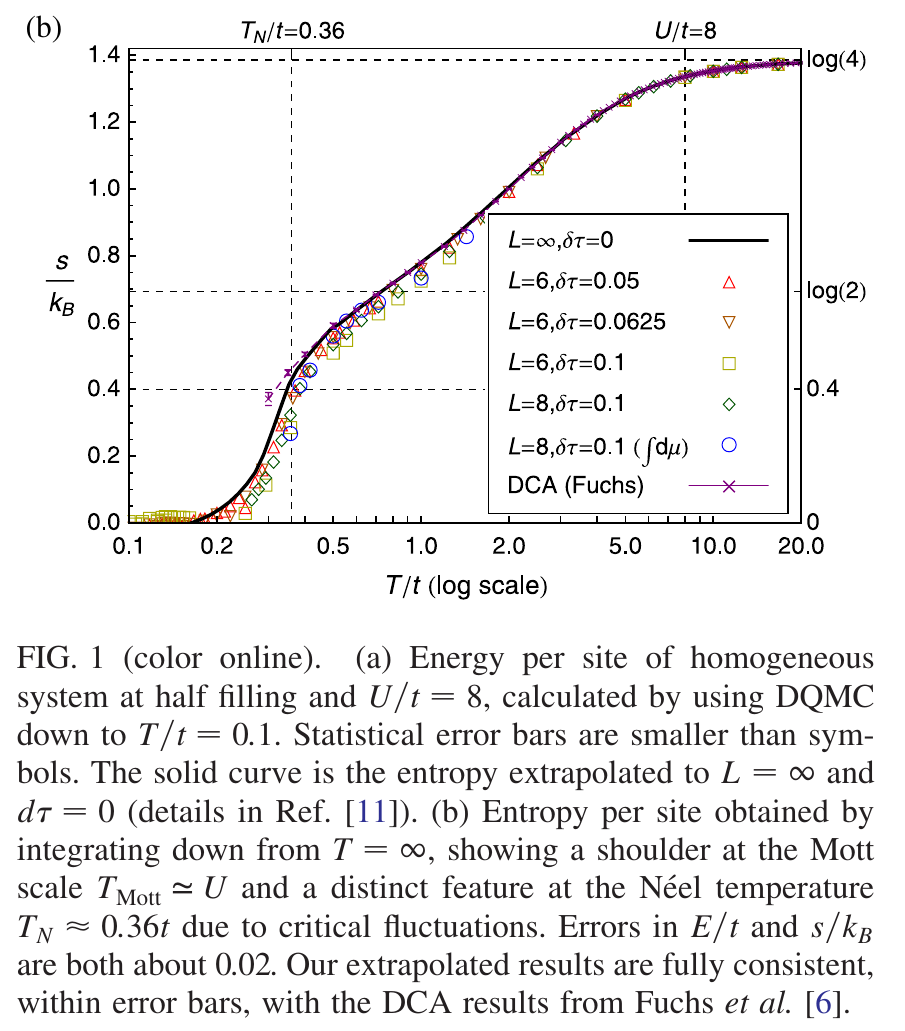
\includegraphics[width=\textwidth]{figures/paiva_entropy.png}
                \caption{Paiva~\cite{Paiva2011}}
                \label{fig:paiva-entropy3D}
        \end{subfigure}
        ~ %add desired spacing between images, e. g. ~, \quad, \qquad etc.
          %(or a blank line to force the subfigure onto a new line)
        \begin{subfigure}[b]{0.48\textwidth}
                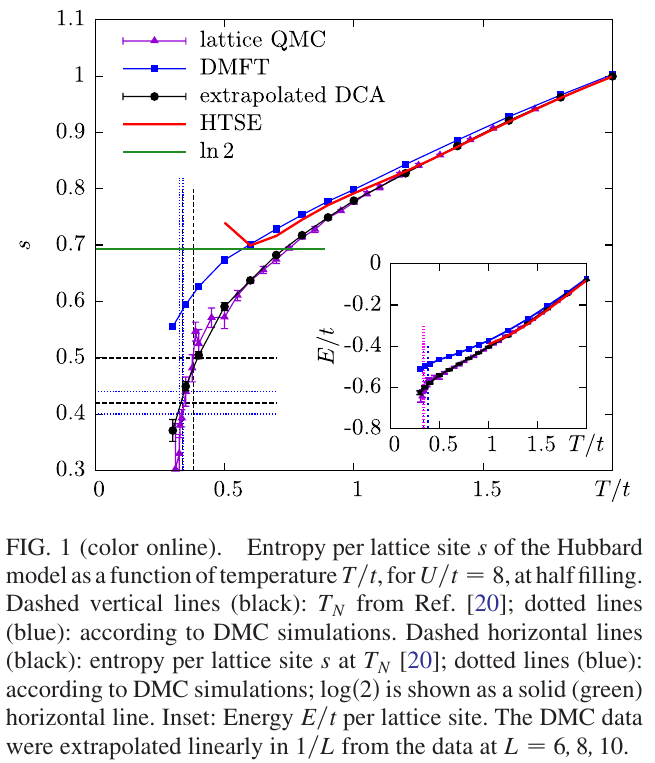
\includegraphics[width=\textwidth]{figures/fuchs_entropy.png}
                \caption{Fuchs~\cite{Fuchs2011}}
                \label{fig:fuchs-entropy3D}
        \end{subfigure}%
        \caption{Calculations of entropy per lattice site versus temperature at half filling.}\label{fig:entropy-Fuchs-Paiva}
\end{figure}
For a homogeneous 3D lattice, at the N\'{e}el temperature $T_{N}=0.36t$, the
entropy per particle is $s=0.4\,\kb$.  As the temperature starts dropping below
$T_{N}$ the entropy approaches zero very quickly in what is referred to as the
AFM transition (AFM stands for antiferromagnetic order).  The AFM transition
has been studied theoretically for homogeneous 3D systems using  quantum
Monte Carlo (QMC)~\cite{Paiva2011} and the dynamical cluster approximation
(DCA)~\cite{Fuchs2011}.  The results from these two approaches are shown in
Figs.~\ref{fig:paiva-entropy3D},\ref{fig:fuchs-entropy3D}.

The theoretical calculations shown correspond to a homogeneous system, but in
practice  one has samples with a finite number of atoms so one is forced to
confine them in order to reach half-filling.   Since the confinement is
typically harmonic (as opposed to a well with hard walls), the density decays
as a function of distance to the center.   We will show below that this
inhomogeneity in the density leads to the concept of entropy redistribution.
We will see that the entropy necessary to achieve a N\'{e}el state can be
higher in a trapped system that in the homogeneous case. 


\subsection{High temperature series expansion for the Hubbard model}

In this section we will plot the thermodynamic properties of the Hubbard model
obtained using the high temperature series expansion (HTSE) to second
order~\cite{Henderson1992,Jordens2010}.   The  HTSE allows us to visualize the
signatures of the Mott insulating state:
\begin{itemize}
   \item The density as function of chemical potential has a plateau at $n=1$
   \item The double occupancy is suppressed 
   \item The density fluctuations are suppressed 
   \item The entropy per site as a function of filling has a dip at $n=1$. 
\end{itemize} 

For the homogeneous Hubbard model, we show in Fig.~\ref{fig:HTSEhomogeneous}
plots of the density,  double occupancy,  density fluctuations and entropy per
site.  We can see the signatures of the Mott state if we look at the variation
of the thermodynamic quantities at $n=1$.  As the temperature gets lower and the
interaction strength is increased these signatures become more pronounced. 
\begin{figure}
        \centering
        \begin{subfigure}[b]{0.75\textwidth}
                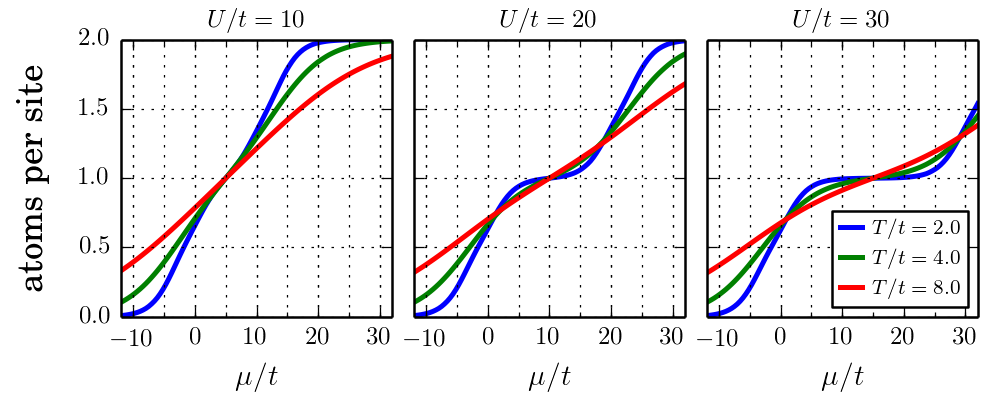
\includegraphics[width=\textwidth]{figures/HTSE_density_U.png}
                \caption{Density}
        \end{subfigure}%
          %add desired spacing between images, e. g. ~, \quad, \qquad etc.
          %(or a blank line to force the subfigure onto a new line)

        \begin{subfigure}[b]{0.75\textwidth}
                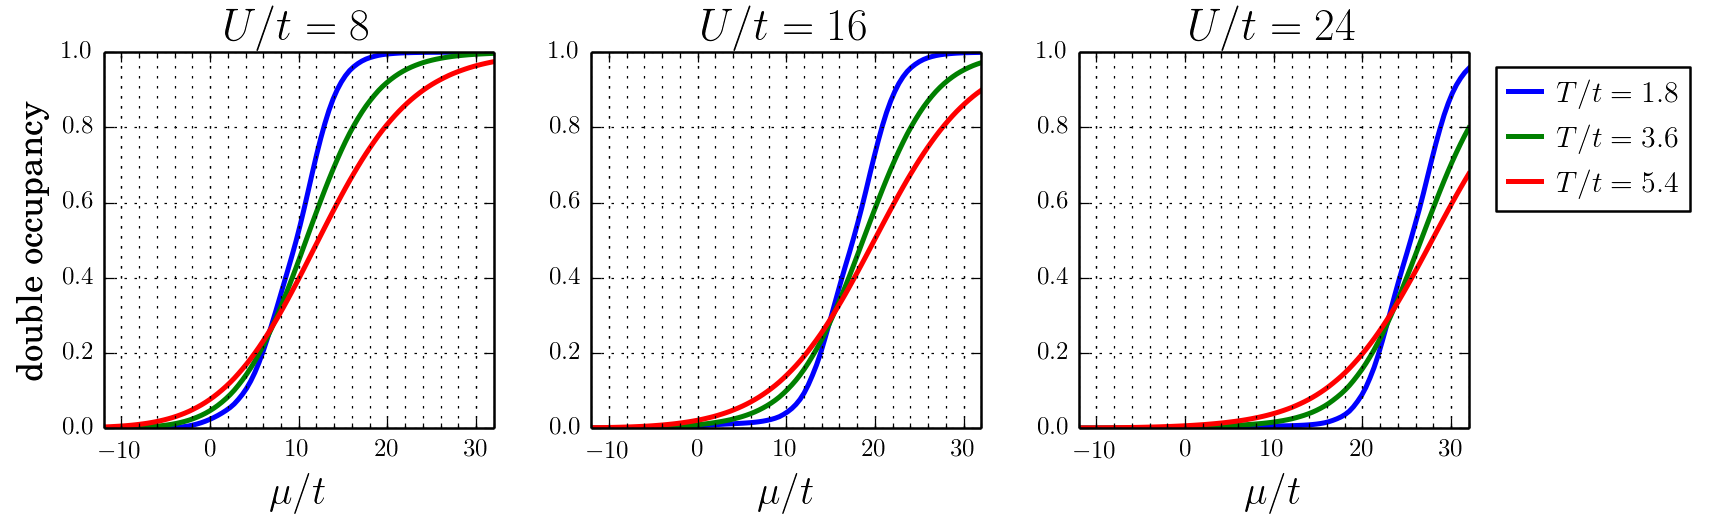
\includegraphics[width=\textwidth]{figures/HTSE_doublons_U.png}
                \caption{Double occupancy}
        \end{subfigure}
 
        \begin{subfigure}[b]{0.75\textwidth}
                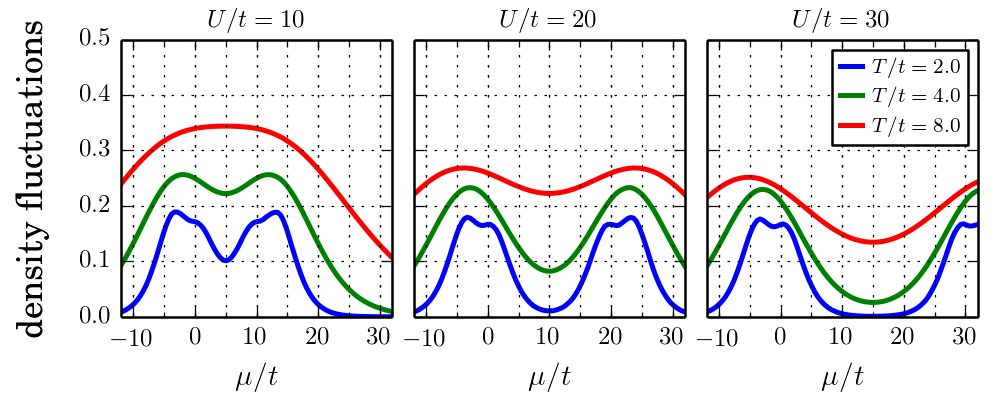
\includegraphics[width=\textwidth]{figures/HTSE_densfluc_U.png}
                \caption{Density fluctuations}
        \end{subfigure}

        \begin{subfigure}[b]{0.75\textwidth}
                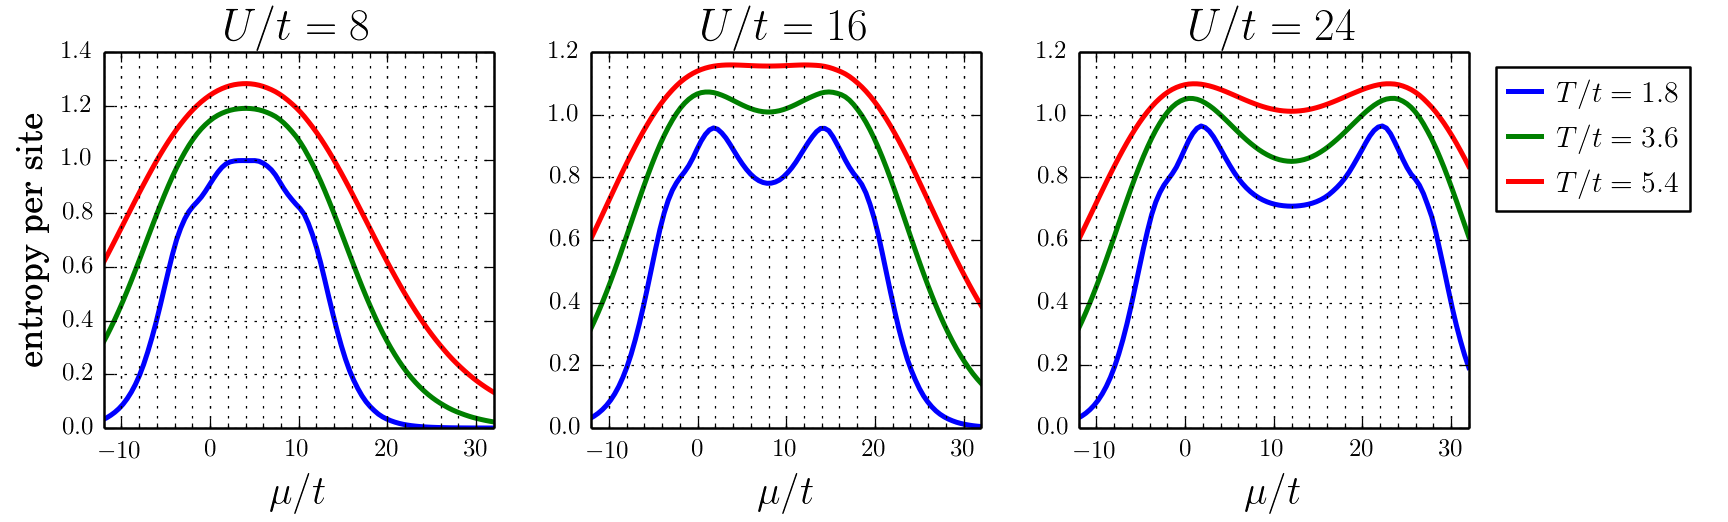
\includegraphics[width=\textwidth]{figures/HTSE_entropy_U.png}
                \caption{Entropy per lattice site}
        \end{subfigure}
        \caption{Thermodynamic quantities as a function of chemical potential calculated using the HTSE.}\label{fig:HTSEhomogeneous}
\end{figure}

\subsubsection{Entropy per particle}  

\begin{figure}
    \centering
    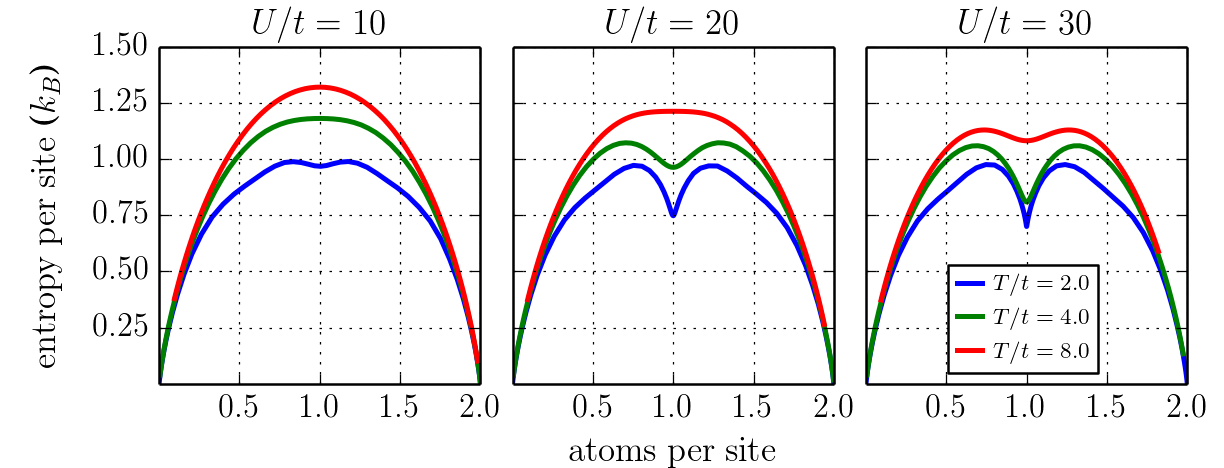
\includegraphics[width=0.8\textwidth]{figures/HTSE_EntropyPerSite_U.png}
    \caption{Entropy per lattice site versus density.}\label{fig:HTSE_spersite}
\end{figure}
The HTSE gives us the result for the entropy per lattice site, which we can
plot versus the density, as shown in Fig.~\ref{fig:HTSE_spersite}  The
interesting result arises if we divide the entropy per lattice site by the
density, in order to obtain the entropy per particle.  This is shown in
Fig.~\ref{fig:HTSE_sperparticle}. 
\begin{figure}
    \centering
    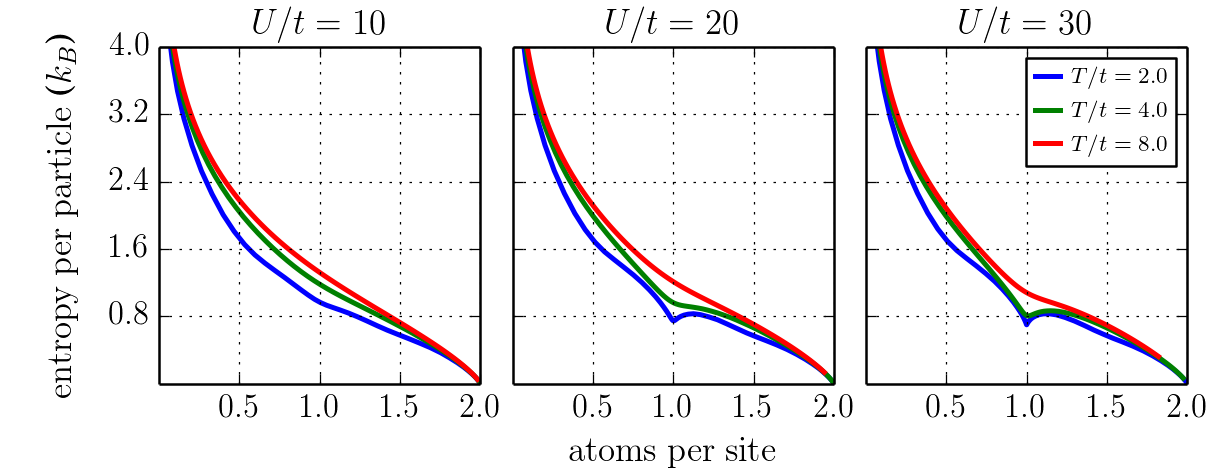
\includegraphics[width=0.8\textwidth]{figures/HTSE_EntropyPerParticle_U.png}
    \caption{Entropy per particle versus density.}\label{fig:HTSE_sperparticle}
\end{figure}
It is seen there that the entropy per particle rises significantly for lower
filling values, and most importantly that the value of the entropy per particle
at low filling \textbf{does not} depend strongly on temperature or interaction
strength.   This property is referred to as the larger entropy capacity of the
metallic shell,  which is at the root of the idea of entropy redistribution. 

\subsection{Local density approximation}

In what follows we will use the results from HTSE and the local density
approximation to calculate trap profiles of the various thermodynamic
quantities.  A trapped gas with a finite number of atoms has a density that
inevitably decreases as a function of distance from the center.   As the
density goes down, the outer shells of the cloud, which are below half-filling,
will have a large entropy per particle.   The overall entropy per particle of
the trapped system, $S/N$, will be distributed such that most of it is carried by
the metallic edges of the cloud.   

\subsubsection{Comparison between a red detuned lattice without and with
compensation}
\label{sec:compare-big-small-waist}

\begin{figure}
        \centering
        \begin{subfigure}[t]{0.48\textwidth}
		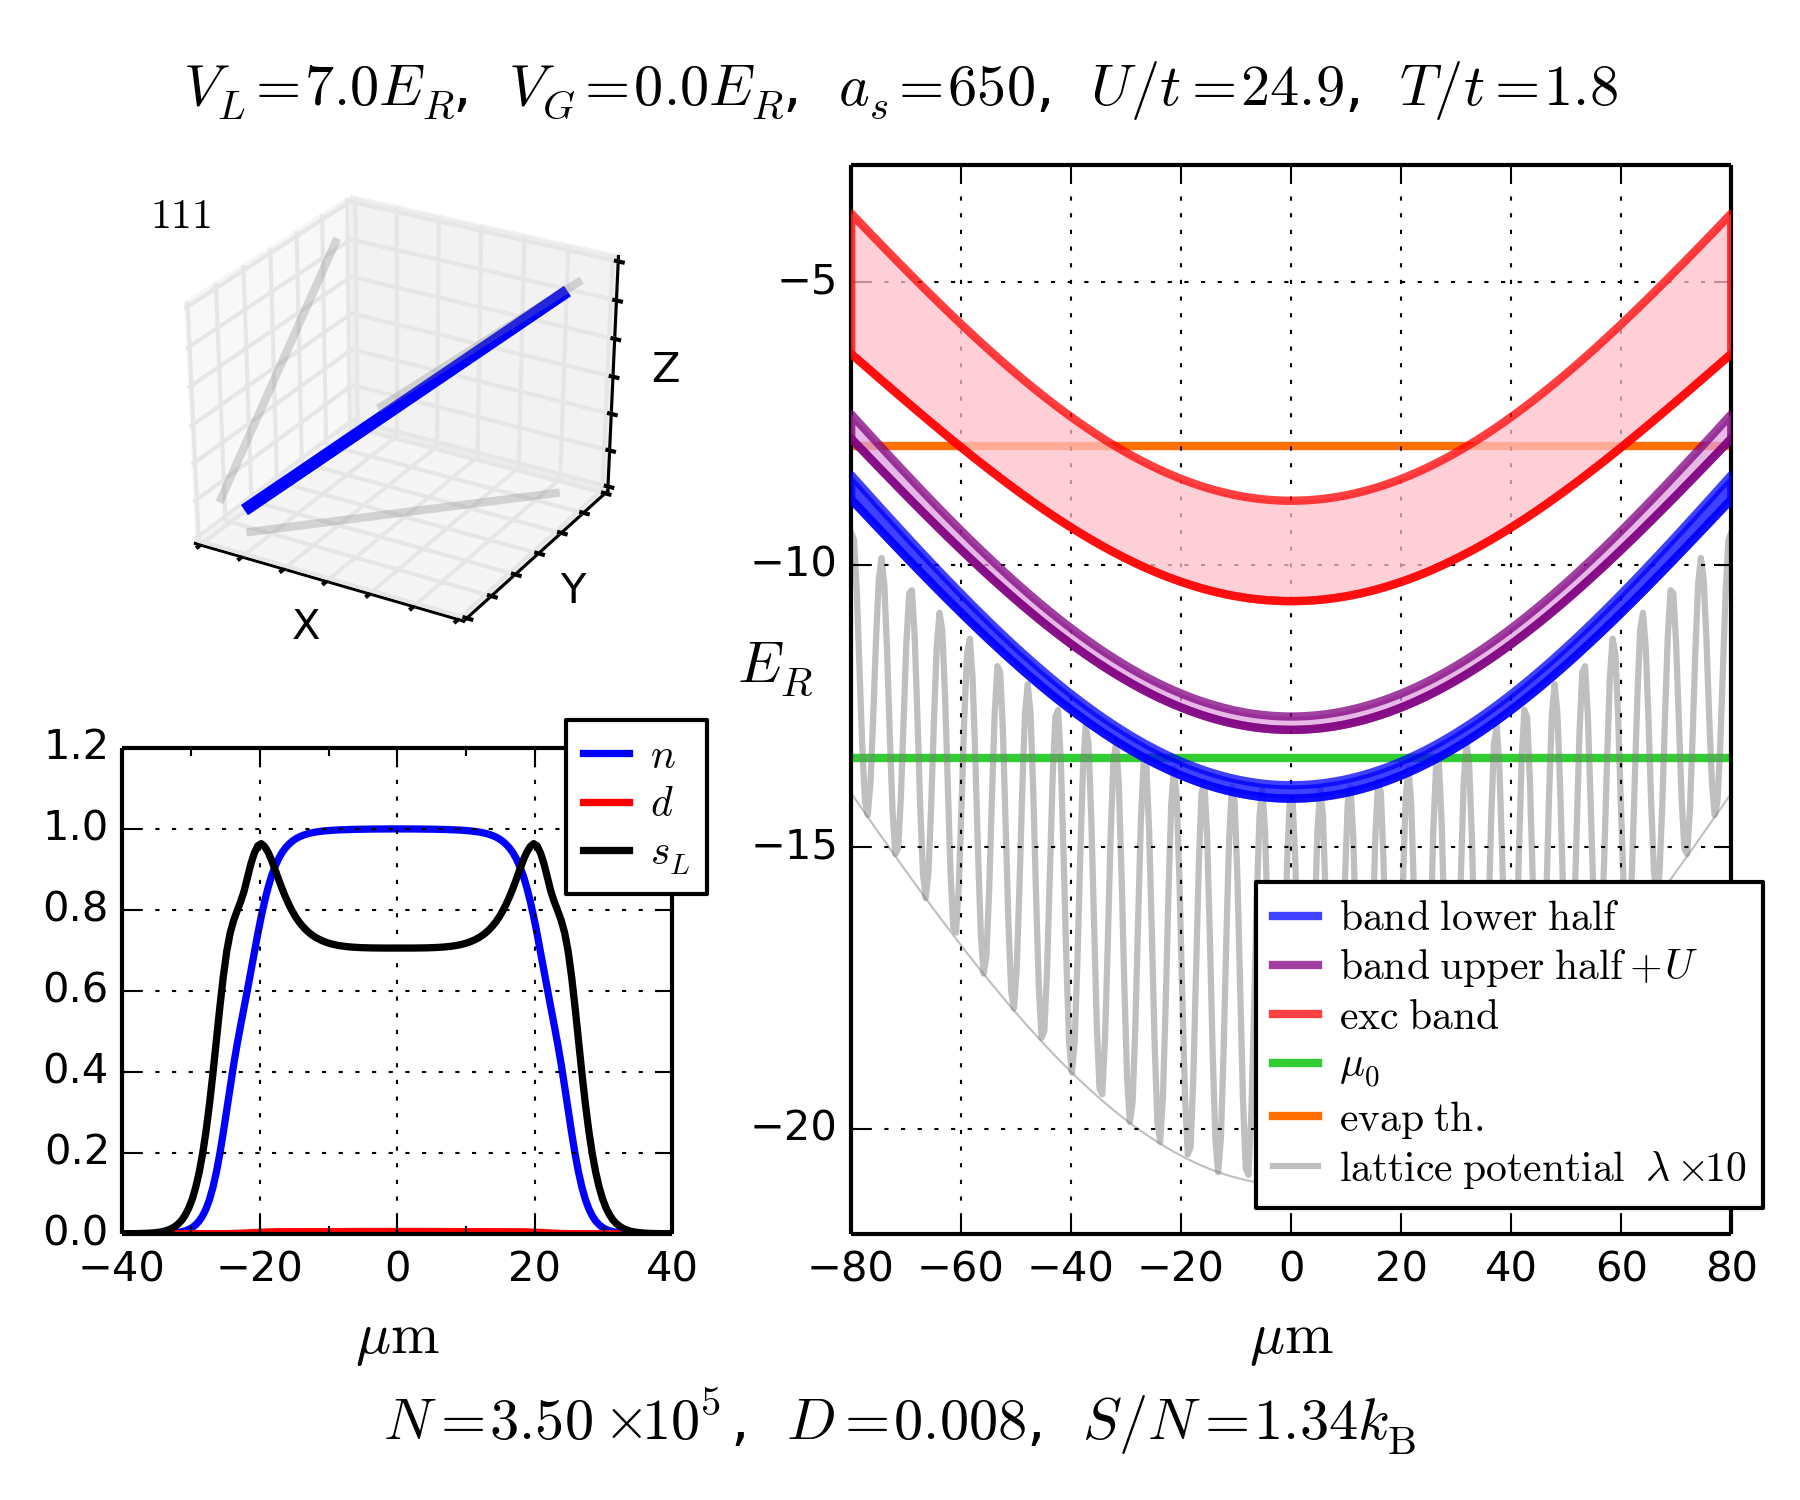
\includegraphics[width=\textwidth]{figures/7Er_red-detuned_no-comp.png}
\caption{Red detuned lattice without compensation.  The lattice beam waist is
146\,$\mu$m for all three lattice axes.  The beam waist is chosen such that the
confinement produces unit filling at the center when there are 350,000 atoms in
the trap. }
                \label{fig:HTSE_full-band-profiles_a}
        \end{subfigure}%
        ~~ %add desired spacing between images, e. g. ~, \quad, \qquad etc.
          %(or a blank line to force the subfigure onto a new line)
        \begin{subfigure}[t]{0.48\textwidth}
		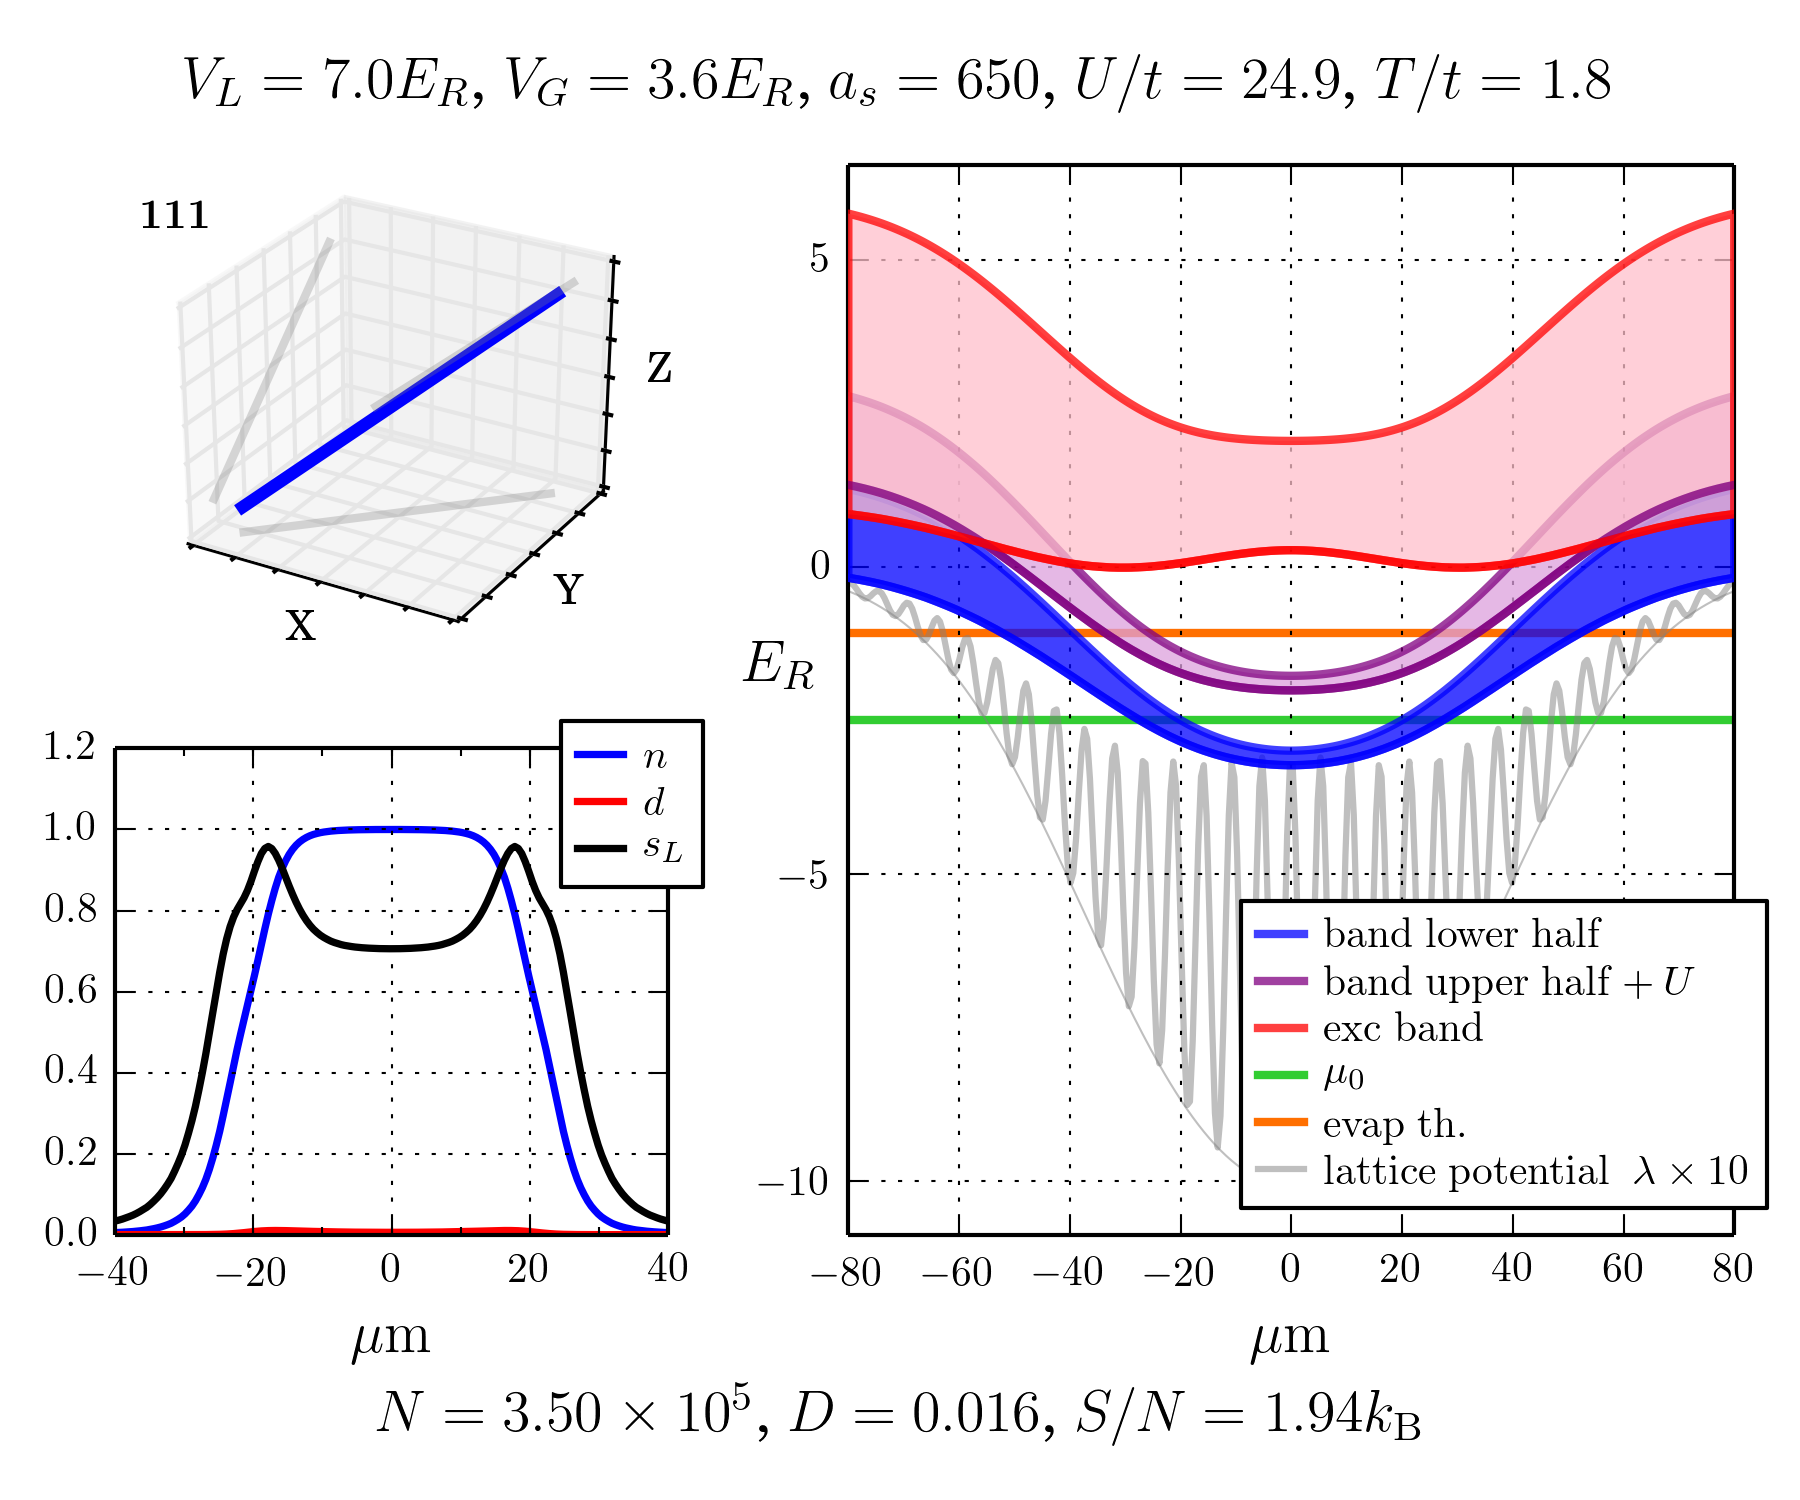
\includegraphics[width=\textwidth]{figures/ir47-gr40_7Er-comp3p642.png}
\caption{Red detuned lattice with compensation.  The lattice beam waist is
47\,$\mu$m and the compensation beam waist is 40\,$\mu$m.  These values are
approximately what we use in our experimental setup.   The compensation depth
of 3.6\,$E_{R}$ is chosen so that unit filling is achieved at the center for an
atom number of 350,000.}
                \label{fig:HTSE_full-band-profiles_b}
        \end{subfigure}
	\caption{Full trap profiles of band structure and thermodynamic
quantities for a lattice without and with compensation.  For both cases the
atom number is chosen to be 350,000 atoms, and the filling at the center is
$n=1$.   Not that despite the very different band structure profiles, the
density profiles are very similar for both cases.  Even though the local
Hubbard parameters and the filling are set to be the same at the center of the
sample, the overall entropy per particle can be 1.5 times larger in the
compensated case (1.94\kb) than in the uncompensated case (1.34\kb). }
\label{fig:HTSE_full-band-profiles}
\end{figure}
Figure~\ref{fig:HTSE_full-band-profiles} shows a comparison of the trap
profiles for a red detuned lattice without compensation
(\ref{fig:HTSE_full-band-profiles_a}) and a red detuned lattice with
compensation (\ref{fig:HTSE_full-band-profiles_b}).    In order to make a
legitimate comparison, we set the atom number to 350,000 atoms.  In the case
without compensation we vary the beam waist of the lattice beams such that a
density of $n=1$ is achieved at the center of the sample.   Lattice beams with
smaller beam waists will produce a stronger confinement, so in general if you
have a large amount of atoms and you want to achieve unit filling without
compensation you must use lattice beams with a large waist.    In the case with
compensation we use the lattice and compensation beam waists that we currently
have in our setup:  $w_{L}=47\,\mu$m and $w_{C}=40\,\mu$m.   We then adjust the
depth of the compensation beams to achieve half filling with 350,000 atoms.  


From looking at this figure we can see that even though the band structure
profiles are very different (in the compensated case the Hubbard parameters
vary strongly with radial distance),  the trap profiles of the density look
very similar in both cases.  Despite this similarity in the density,  the
double occupancy and the entropy per lattice site are slightly different.   The
important result is that even though in both cases one has the exact same local
state at the center (same filling, same $U/t$, same $s$)  the overall entropy
per particle can be larger for the compensated lattice by a factor of 1.5
(1.94\kb to 1.34\kb).   

This larger capacity of the compensated lattice to redistribute entropy is what
can make it favorable to achieve an AFM ordered state at the center of the
sample.   If one looks in more detail, as is shown in
Fig.~\ref{fig:HTSE_compare-thermo} one realizes that the larger entropy
capacity comes from a small enhancement of the double occupancy ( on the half-a
percent level ) which leads to a slightly larger entropy per particle on the
region from about 5\,$\mu$m to 25\,$\mu$m radius.   This radii encompass a
large volume of the trap, which can make a difference on the overall entropy
capacity even though the extra entropy per particle plotted radially looks very
small.  
\begin{figure}
    \centering
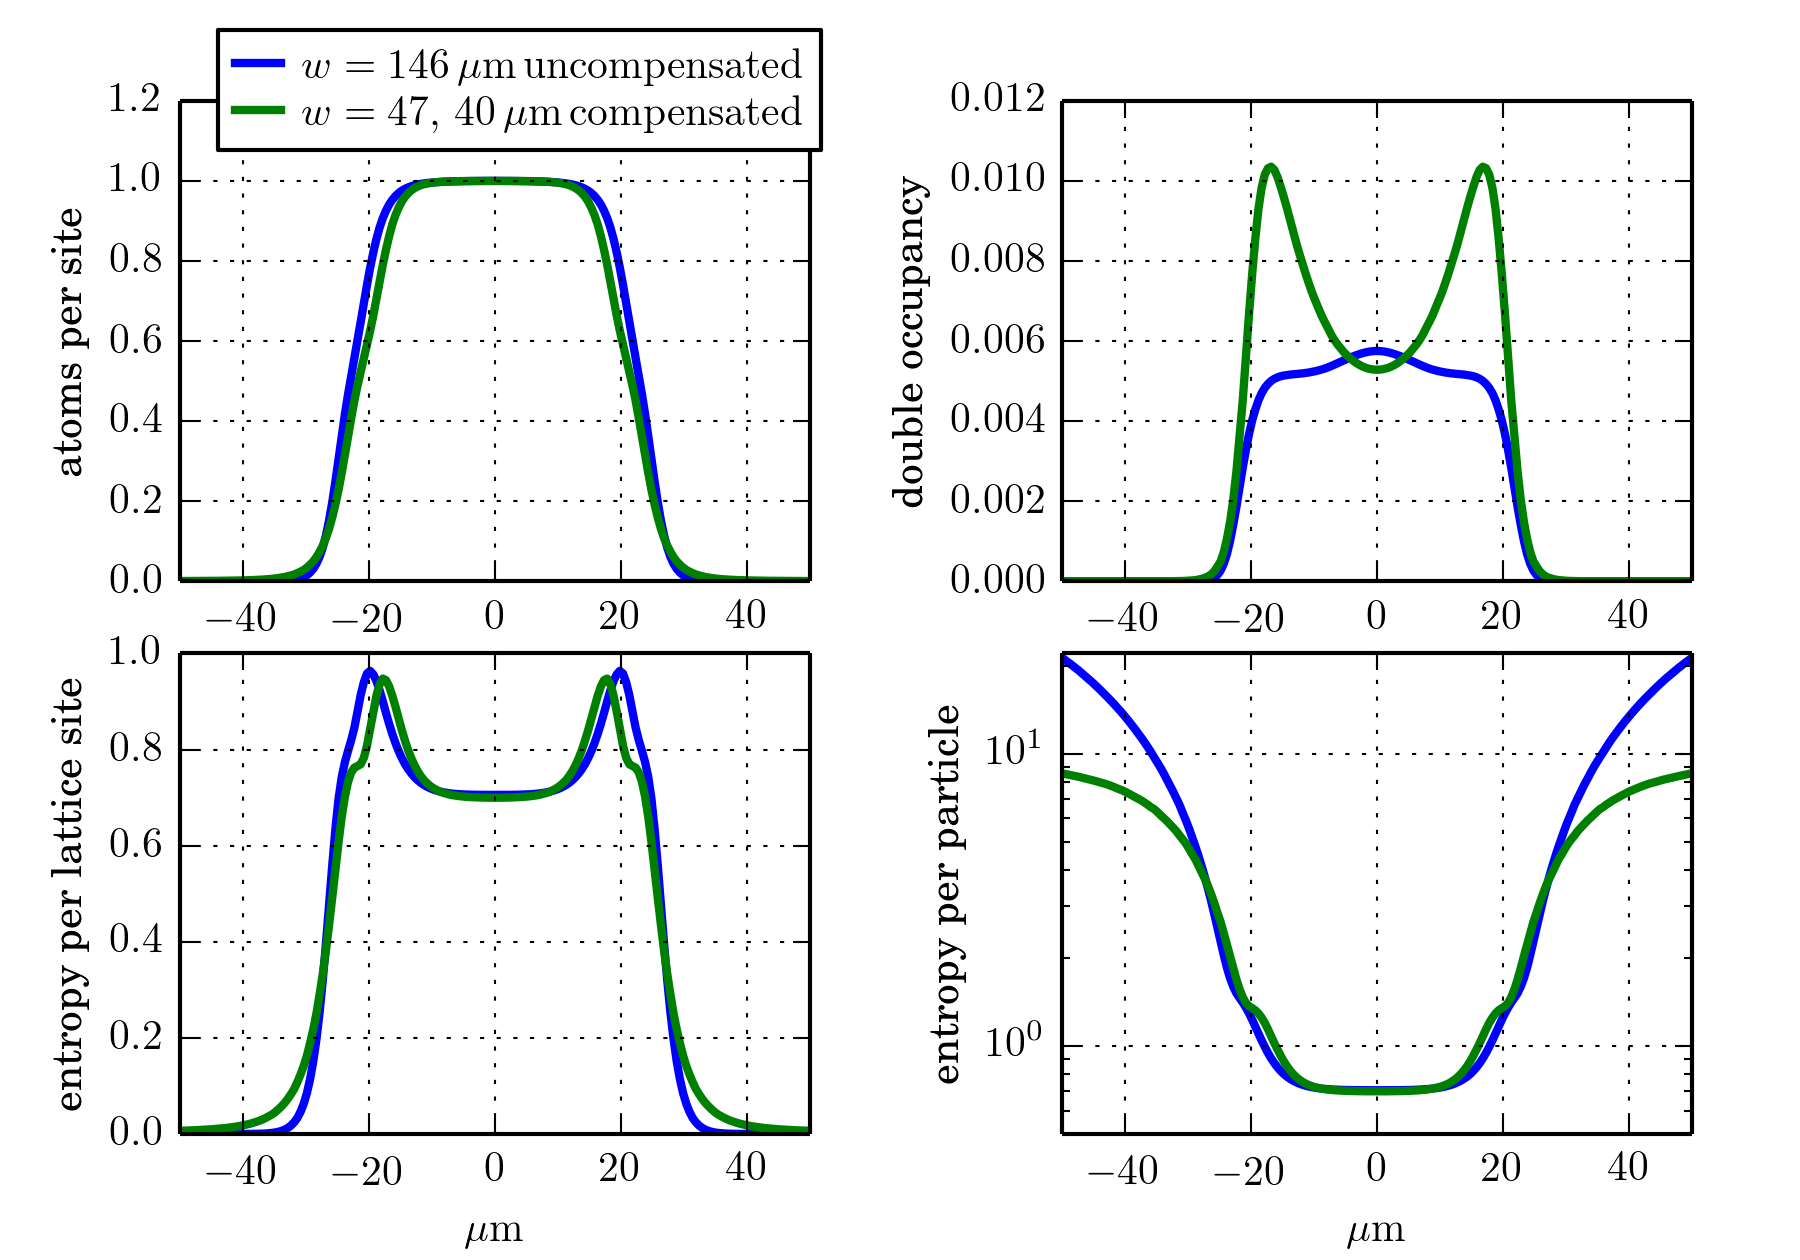
\includegraphics[width=0.65\textwidth]{figures/HTSE_compare-thermo.png}
\caption{Detailed comparison of the thermodynamic quantities for the large beam
waist uncompensated lattice and the small beam waist compensated lattice.  The
density is very similar for both cases.  The double occupancy is quite
different, which leads to a very slightly larger entropy per particle across a
large range of radii in the trap. }\label{fig:HTSE_compare-thermo}
\end{figure}


The profiles that are shown in Fig.~\ref{fig:HTSE_full-band-profiles} are
calculated at a temperature $T=1.8t$, which is near the lowest temperature
value accessible with the HTSE.   The chemical potential, measured from the
lowest energy level available to the system (the bottom of the band) is set to
$\mu=6t +U/2$ to guarantee half-filling at the center.  \footnote{ The $6t$
here is half the bandwidth.  Note that in typical treatments the chemical
potential is always measured from the center of the lowest band, so the $6t$
will be omitted. In that case the chemical potential associated with
half-filling Will be $U/2$.  Some treatments even shift the zero of energy by
$U/2$ so that half filling occurs nominally at $\mu$=0 regardless of $U$. } We
used a value of $U=24.9t$,  given by the scattering length, which is set at
650$a_{0}$.   

Plugging in these values we obtain $\mu\approx 18 t$  or $T/\mu \approx 1.8/18
= 0.1 $.  When the temperature is so low, one can safely assume that $\mu
\approx E_{F}$,  so this system would have  $T/T_{F}=0.06$ at an overall
entropy per particle of $S/N=1.94\kb$.  If the sample was obtained by ramping
up the lattice adiabatically starting from a harmonic trap, then the initial
entropy in the harmonic trap should also be 1.94\kb.  In the harmonic trap this
corresponds to $T/T_{F} = S/(\pi^{2} N) \approx 0.2$.  

We conclude from these rough estimates that as the sample gets loaded into the
lattice it gets adiabatically cooled, its value of $T/T_{F}$ is reduced.  This
is in contrast with the result obtained in~\cite{Kohl2006} where it was
concluded that loading a gas adiabatically from a harmonic trap to a deep
optical lattice would adiabatically heat the gas.   In this case we are
considering interactions and not neglecting the width of the lowest band.  Our
observation that the gas is adiabatically cooled as it is loaded into the
lattice are consistent with the results from~\cite{Paiva2011}.   

(NOTE: I NEED TO ASK THEREZA ABOUT THESE REMARKS TO CHECK THAT I AM NOT MAKING
A MISTAKE. 

The main question is whether it is ok to take $\mu=E_{F}$ since $\mu$ is in
the Mott gap.   Should one take  $E_{F}=12t$ in that case, since the top of the
band is the largest energy state that could potentially be occupied?? )


\subsubsection{ Enlarging the Mott state}  

In this section we consider our experimental setup
($w_{\text{L}}=47\,\mu\mathrm{m}$, $w_{\text{C}}=40\,\mu\mathrm{m}$)  and we
vary the amount of compensation.   What we find is that if no compensation is
used, then the number of atoms has to be very small in order to achieve
half-filling at the center.     On the other hand,  when using compensation one
can still hold a large number of atoms and maintain half-filling.   This leads
to the concept of enlarging the Mott state ( or N\'{e}el state if your
temperature is low enough)  which can be a very dramatic effect as was shown in
the paper by Mathy, Huse and Hulet~\cite{Mathy2012}.  

The effect of enlarging the Mott state is shown in
Fig.~\ref{fig:HTSE_enlarge-mott}, where we show the relationship between atom
number and compensation when the filling is set to $n=1$ at the center of the
cloud. This figure also shows the profile plots for no compensation and a
compensation of 3.05\,$E_{R}$,  in order to illustrate how the Mott plateau in
the density profile is enlarged for larger compensation.  
\begin{figure}
        \centering
        \begin{subfigure}[t]{0.32\textwidth}
		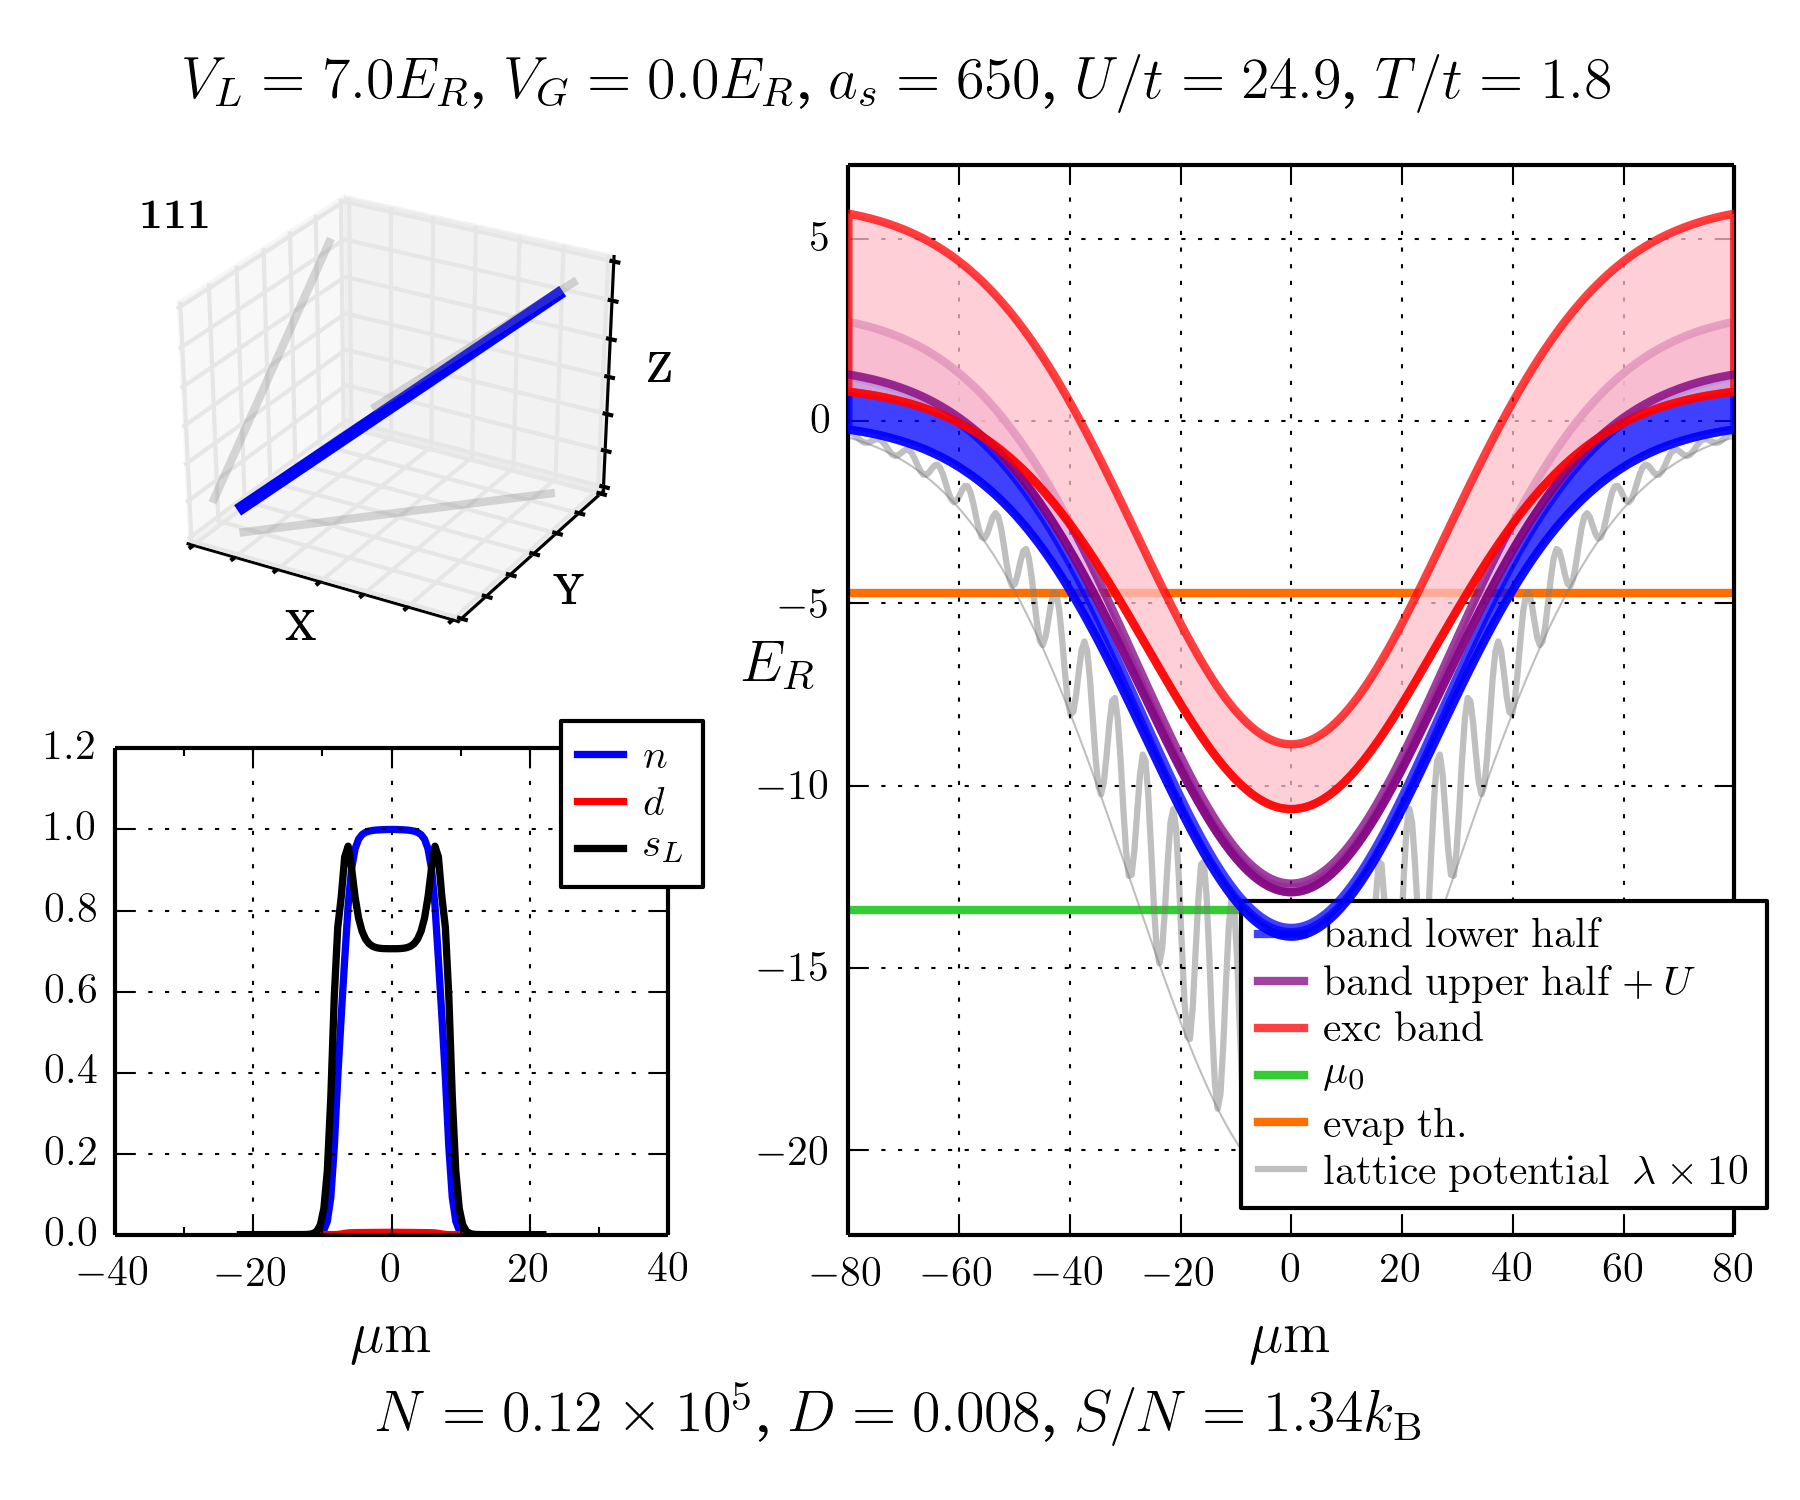
\includegraphics[width=\textwidth]{figures/ir47-gr40_7Er-comp0p0.png}
\caption{$w_{L}=47\,\mu$m and $w_{C}=40\,\mu$m without compensation.  }
                \label{fig:HTSE_enlarge-mott_a}
        \end{subfigure}%
        ~ %add desired spacing between images, e. g. ~, \quad, \qquad etc.
          %(or a blank line to force the subfigure onto a new line)
        \begin{subfigure}[t]{0.32\textwidth}
                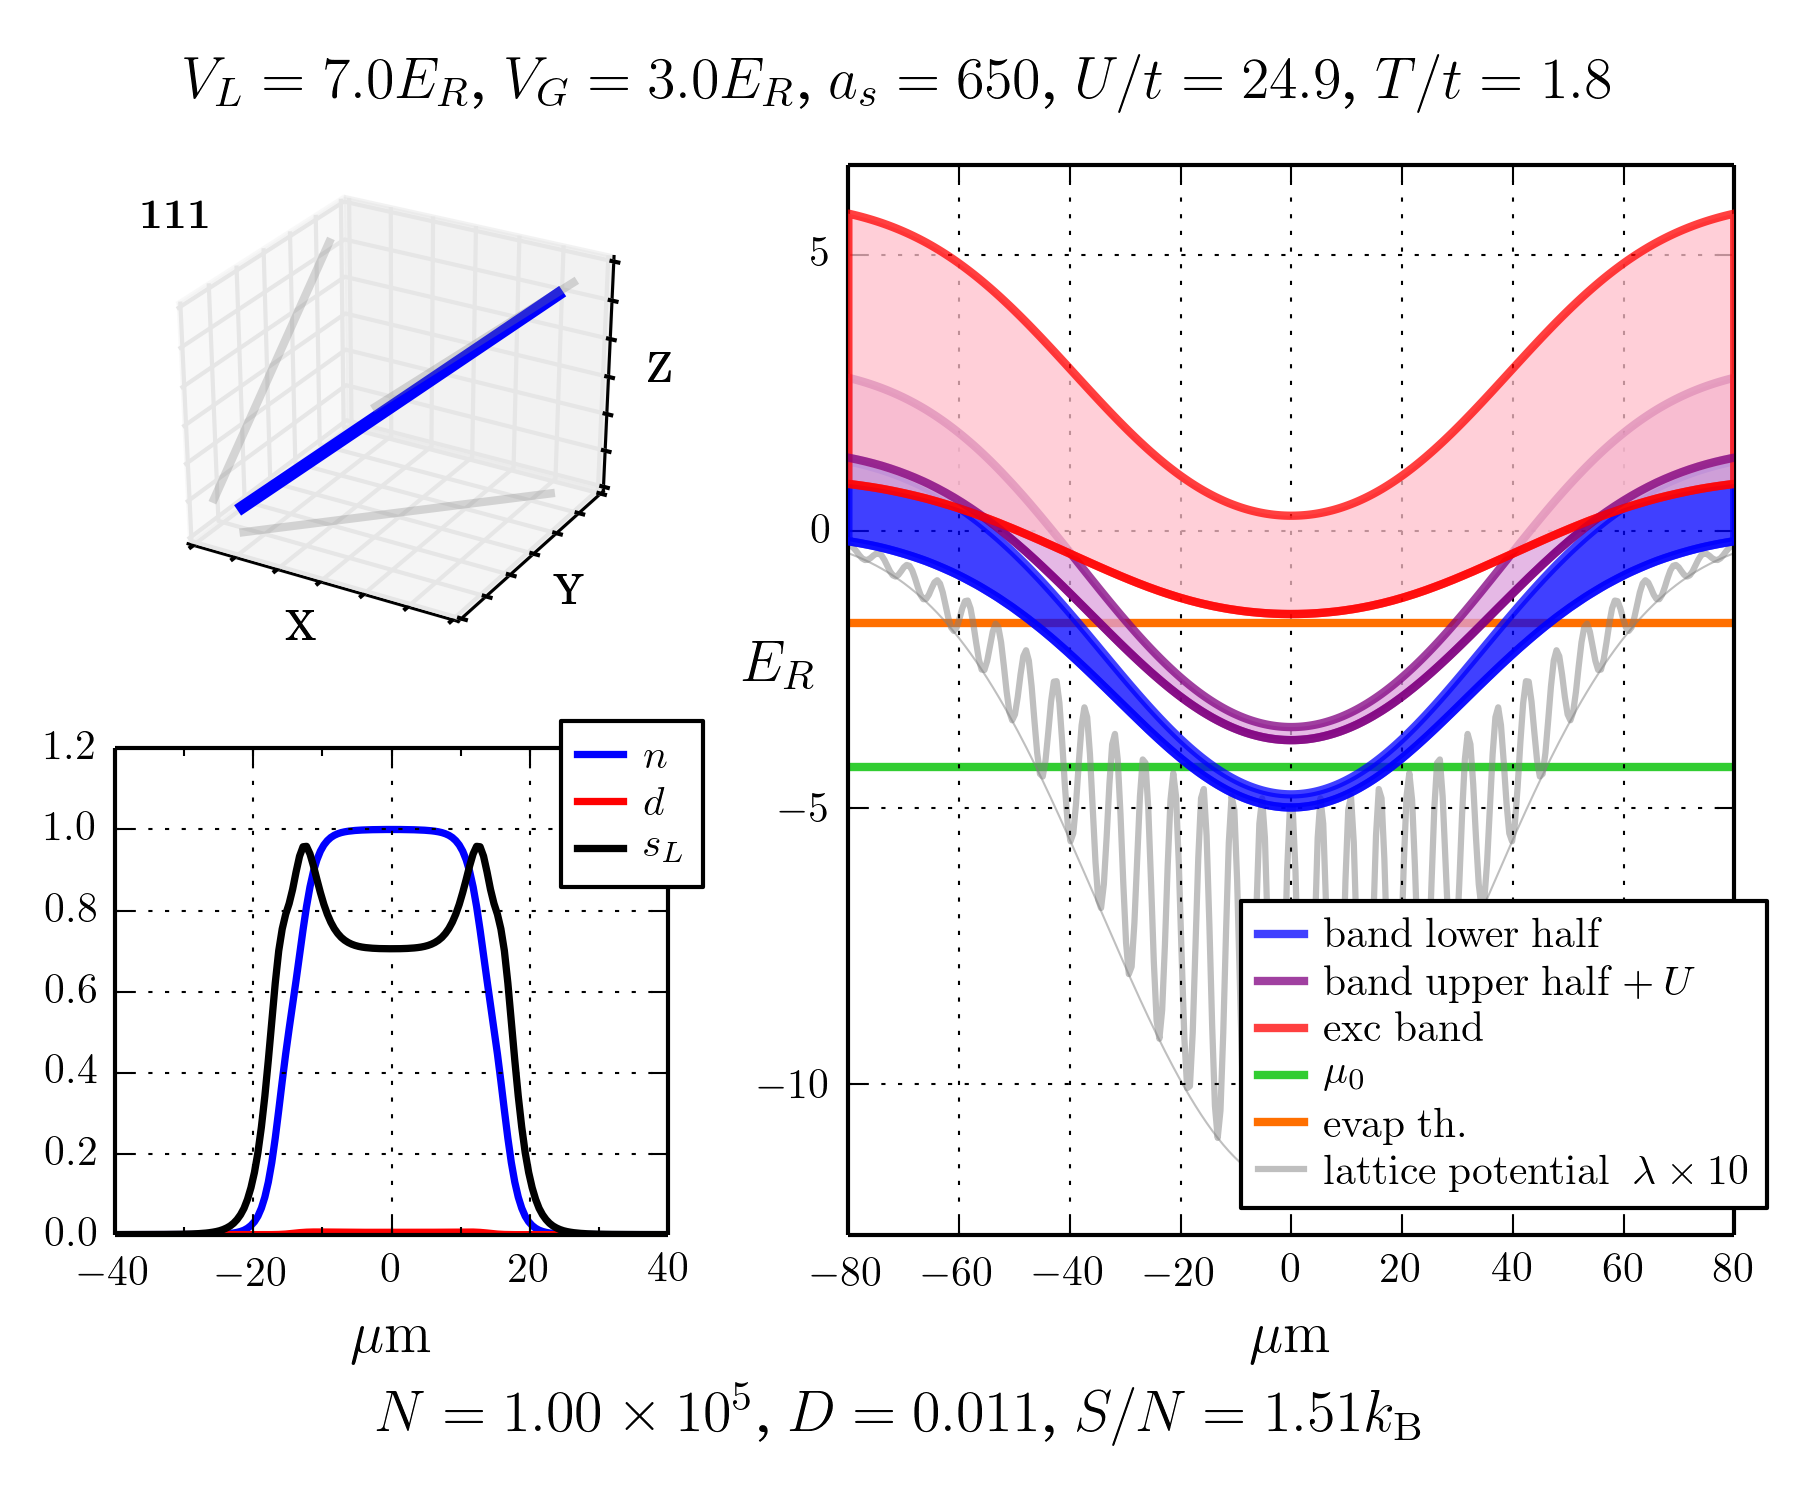
\includegraphics[width=\textwidth]{figures/ir47-gr40_7Er-comp3p05.png}
\caption{$w_{L}=47\,\mu$m and $w_{C}=40\,\mu$m with 3.05\,$E_{R}$ compensation.  }
                \label{fig:HTSE_enlarge-mott_b}
        \end{subfigure}
        ~        
        \begin{subfigure}[t]{0.32\textwidth}
                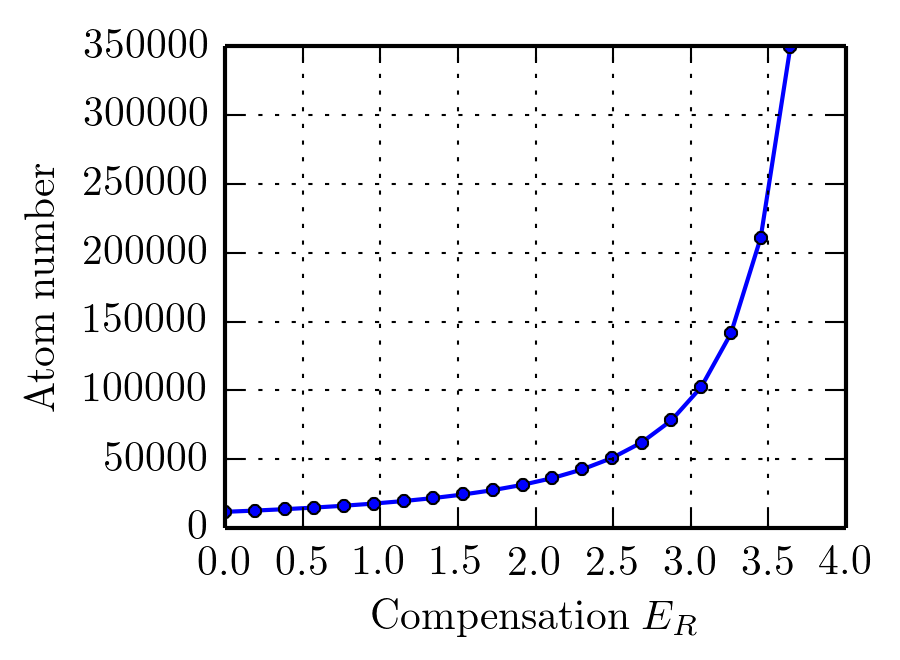
\includegraphics[width=\textwidth]{figures/enlarging_mott_state.png}
\caption{Atom number as a function of compensation illustrates the concept of enlarging the Mott state. }
                \label{fig:HSTE_enlarge-mott_c}
        \end{subfigure}
	\caption{  Illustrating the idea of enlarging the Mott state. 
}
\label{fig:HTSE_enlarge-mott}
\end{figure}


From what was discussed in \S\ref{sec:compare-big-small-waist}  we see that it
is also possible to reach an large Mott plateau for $N=350,000$ and without
compensation beams:  you just need to have larger lattice beam waists.  As we
saw there, the advantage of realizing the large Mott plateau with small lattice
beam waists and compensating beams is  that this system has a larger entropy
capacity  than the large-beam-waist-uncompensated counterpart.   

In addition to this entropy capacity advantage, the
small-beam-waist-compensated setup offers the possibility of evaporative
cooling since the chemical potential comes much closer to the energy threshold
for an atom escaping along one of the lattice beams.  We will address this
point in the following section.  


\section{ Evaporative cooling in a lattice }

If we refer back to Fig.~\ref{fig:HTSE_full-band-profiles}  we can see that on
the energy landscape plot we used an orange line to indicate the evaporation
threshold, that is the energy necessary for an atom to escape along one of the
lattice beams.  Comparing the two cases one sees that the small beam waist
compensated case has a global chemical potential (green line) that is much
closer to the evaporation threshold.

When evaporative cooling a thermal gas of atoms, one considers the parameter
$\eta=U_{\text{trap}}/\kb T$, where $U_{\text{trap}}$ is the energy threshold
for a particle leaving the trap (i.e. the trap depth) and $T$ is the
temperature of the gas.   The evaporation rate is suppressed by a factor
$\exp(-\eta)$ where  typically $\eta\sim10$ and, as the gas cools down, the trap
depth is reduced to force further evaporation~\cite{OHara2001}.  

For a deeply degenerate Fermi gas,  $T \ll T_{F}$, the evaporation rate is
given by~\cite{OHara2001}.
\begin{equation}
  \Gamma_{\text{evap}} \propto \gamma_{\text{coll}} \frac{T}{T_{F}} 
  \exp\left[ -   
  \frac{ U_{\text{trap}} - \kb T_{F} }{ \kb T }  \right ] 
\end{equation}
where $\gamma_{\text{coll}}$ is the classical collision rate evaluated at the
Fermi surface.  This can also be written as 
\begin{equation}
  \Gamma_{\text{evap}} \propto \gamma_{\text{coll}} \frac{T}{T_{F}}
  \exp\left[ \frac{1}{T/T_{F}} \right]  
  \exp\left[ -  \frac{1}{T/T_{F}} \left( \frac{U_{\text{trap}}}{\kb T_{F}} \right) \right] 
\end{equation}
We define $ \eta_{F} \equiv U_{\text{trap}}/\kb T_{F}$ and observe that 
\begin{equation}
  \Gamma_{\text{evap}} \propto \gamma_{\text{coll}} \frac{T}{T_{F}}
  \exp\left[ -  \frac{\eta_{F} - 1 }{ T/T_{F} } \right]
\end{equation}
For the deeply degenerate gas, the $\eta$ factor which determines the
exponential suppression of the evaporation due to the trap depth is effectively
\begin{equation}
 \eta = \frac{\eta_{F} - 1 }{T/T_{F} } 
\end{equation}
Notice that the evaporation rate is additionally suppressed by a factor
$T/T_{F}$ due to Pauli blocking of one of the final states of a collision, which
occurs for $T\ll T_{F}$~\cite{OHara2001}.

We start by considering a red-detuned lattice with no extra confinement or
compensation.  We set  $n=1$ at the center of the sample and vary the waist of
the lattice beams.    From our knowledge of the potentials we can determine
$U_{\text{trap}}$, which in this case is the energy required for an atom to
escape along one of the lattice beams.   At a temperature of $T=1.8t$  we can
make the approximation $\kb T_{F} \approx \mu$, where $\mu$ is the global
chemical potential.  Figure~\ref{fig:etaF-no-comp_vary-wIR} shows $\eta_{F}$ as
a function of lattice beam waist, and also shows the number of atoms
required to achieve half-filling.   
\begin{figure}
    \centering
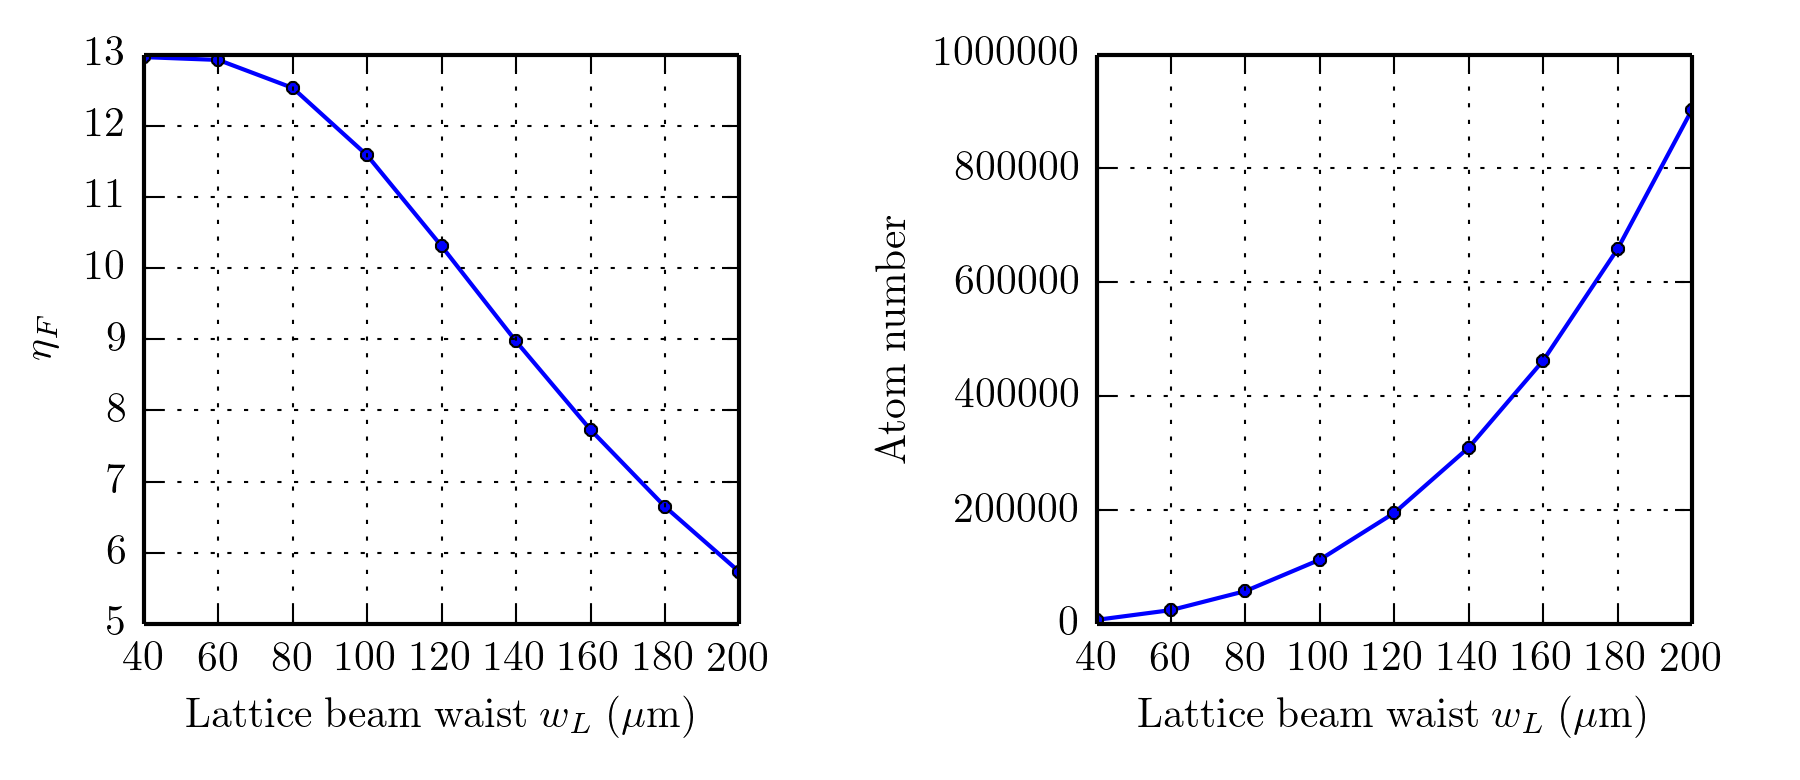
\includegraphics[width=0.8\textwidth]{figures/etaF-no-comp_vary-wIR.png}
\caption{$\eta_{F}$, an indicator of the exponential suppression of evaporation
is shown as a function of lattice beam waist for a red-detuned lattice without
any extra confinement or compensation. To determine $\eta_{F}$ the number of
atoms is adjusted such that filling is $n=1$ at the center.   The required
number is shown on the right.}\label{fig:etaF-no-comp_vary-wIR}
\end{figure}

In our experiment we can produce cold samples with $\sim$350,000 atoms.   As
can be seen in Fig.~\ref{fig:etaF-no-comp_vary-wIR} (and also was already shown
in Fig.~\ref{fig:HTSE_full-band-profiles_a}),  using a beam waist of
146\,$\mu$m would produce the confinement necessary to reach half-filling at
the center with $N=350,000$.  The flip side of this is that, for that beam
waist $\eta_{F}$ would be $\approx 8.5 $,  which for $T/T_{F}=0.1$ means that
the rate of evaporation would be suppressed by  
\begin{equation}
   \frac{T}{T_{F}}\exp\left[ - \frac{\eta_{F} - 1 }{T/T_{F} } 
 \right] \equiv \xi_{\text{evap}}\approx 10^{-34} 
\end{equation} 

Going back to our current setup, which has $w_{L}=47\,\mu$m and
$w_{C}=40\,\mu$m,  with 350,000 atoms; we can achieve half filling if we use
3.64$E_{R}$ of compensation.  This yields $\eta_{F} \approx 2.95$.  This is a
lot better than the large-beam-waist-uncompensated case, however the suppression
factor for the rate of evaporative cooling is still very small.  For our
current setup it would be
\begin{equation}
 \xi_{\text{evap}} = 3.4\times 10^{-10} 
\end{equation}

Under typical evaporation conditions $\eta=10$, and for a non-degenerate sample
we have 
\begin{equation}
 \xi_{\text{evap}} = e^{-10} = 4.5\times 10^{-5} 
\end{equation}
We conclude that our current setup would  have an evaporation rate \textbf{five
orders of magnitude smaller} compared to the typical evaporative cooling rate
for a thermal gas (given the same rate of elastic collisions
$\gamma_{\text{coll}}$).   In addition, in order to get a more realistic
estimate we would need to incorporate the implications of the chemical
potential being in a gapped region of the spectrum (for half-filling the chemical
potential is at the center of the Mott gap) which should further reduce the
evaporation rate.  

We now explore the entire parameter space, where we allow the lattice and
compensation beam waists to vary.   We set the chemical potential so that $n=1$
at the center of the sample,  we do this because half-filling is a prerequisite
to achieve Mott or N\'{e}el states.   We attempt to find a compensation such
that $N=350,000$ atoms.  For some values of the beam waists that is not
possible because it would lead to either spilling atoms from the
trap\footnote{In cases when $w_{C}>w_{L}$.} or to the creation of a negative
curvature in the confinement at the center of our sample\footnote{In cases when
$w_{C} < w_{L}$.  We also refer to this as making a donut}.  
\begin{figure}
    \centering 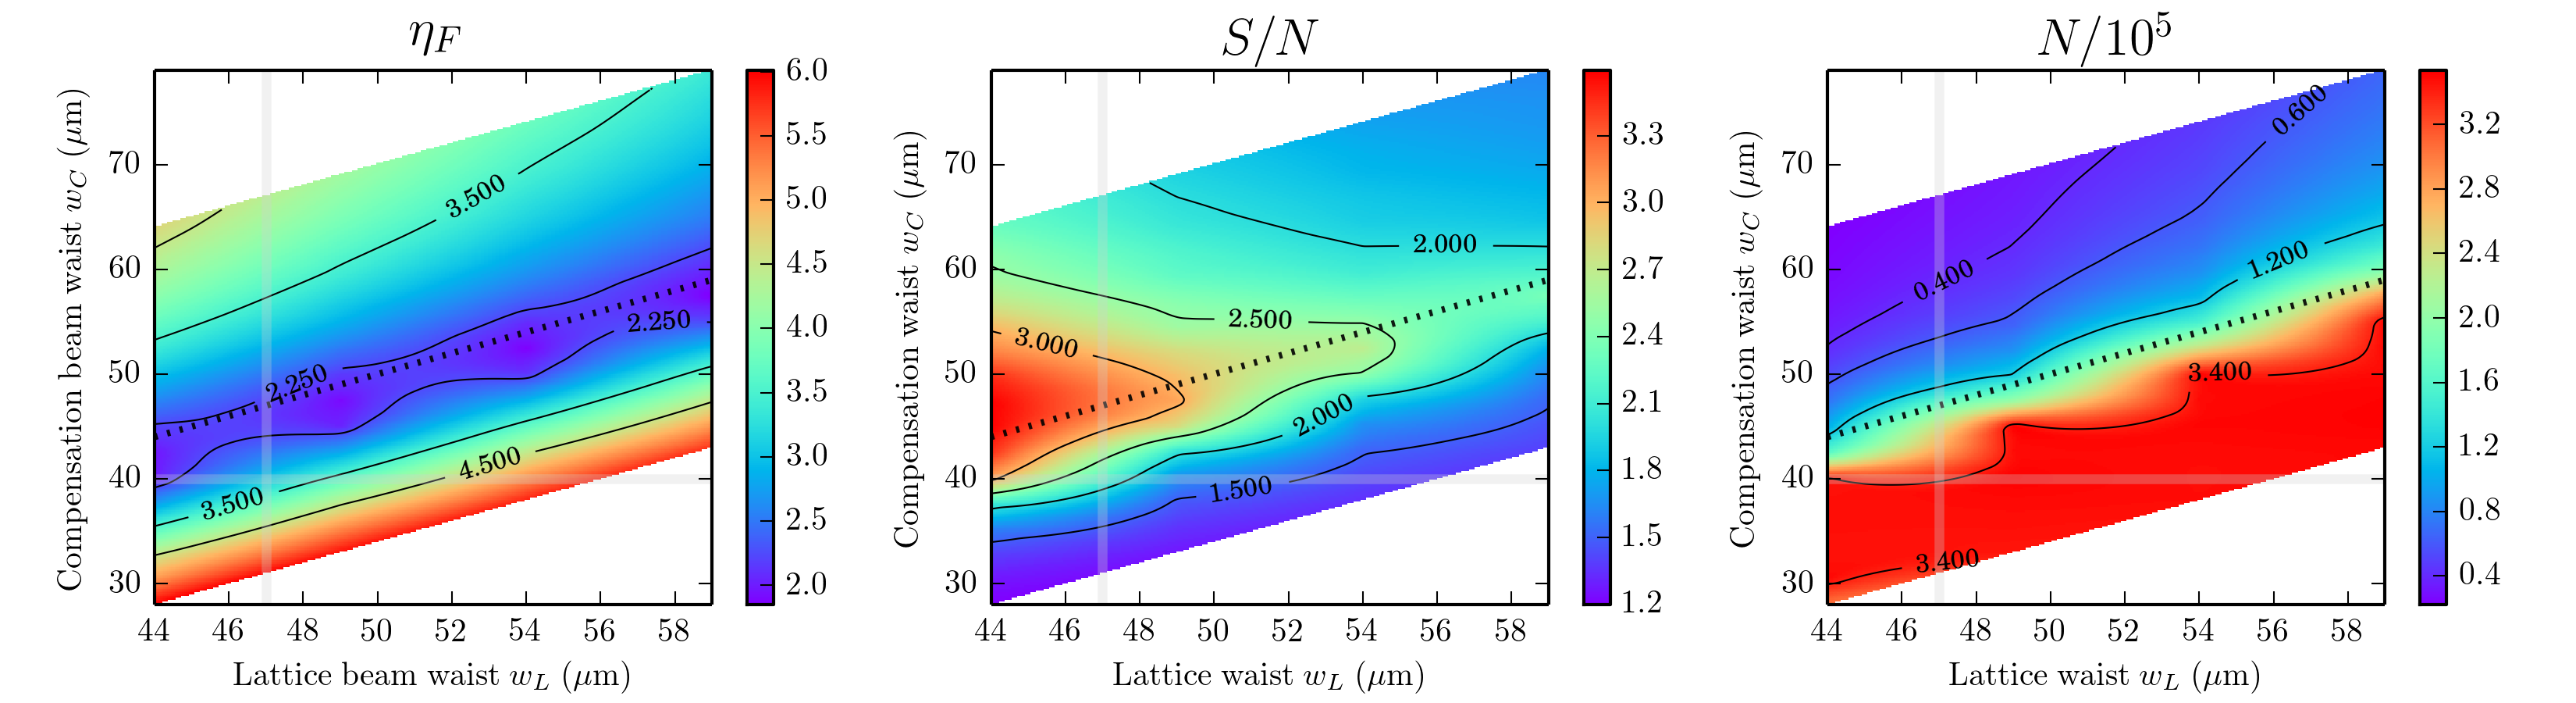
\includegraphics[width=\textwidth]{figures/etaF-wIRwGR.png}
\caption{$\eta_{F}$ and $S/N$ and $N$ are plotted for various lattice and
compensation beam waists.  The filling is set to $n=1$ at the center. The
compensation depth is adjusted so that  $N=350,000$ if it is possible, otherwise
it is set to maximize the atom number without spilling any atoms form the trap
or creating a Mexican hat at the center of the potential.  The dotted line in
the plots corresponds to $w_{L}=w_{C}$.  The current values of our
experimental setup are shown as gray lines,  such that the intersection between
these two gray lines represents our current conditions. }
\label{fig:etaF-wIRwGR}
\end{figure}

The results of the
exploration of the beam waist parameter space are shown in
Fig.~\ref{fig:etaF-wIRwGR}.  The main points that stand out are
\begin{itemize}
\item  An optimal value of $\eta_{F}$ is achieved for $w_{L}\approx w_{C}$.  
\item  At $w_{L} \approx w_{C}$, smaller beam waists give better entropy capacity 
\item The atom number can only reach 350,000 if $w_{C} < w_{L}$, such as in our
current setup.  Otherwise the atom number is limited, being smaller for larger
$w_{C}$.
\end{itemize}


To get another look at the results, on Fig.~\ref{fig:etaF-wIRwGR-lines} we plot
$\eta_{F}$, $S/N$, and $N$  as a function of $w_{C}$ for three different values
of $w_{L}$.  The evaporation factor is optimized for nearly equal beam waists
and the entropy capacity also peaks up around there. 
\begin{figure}
    \centering
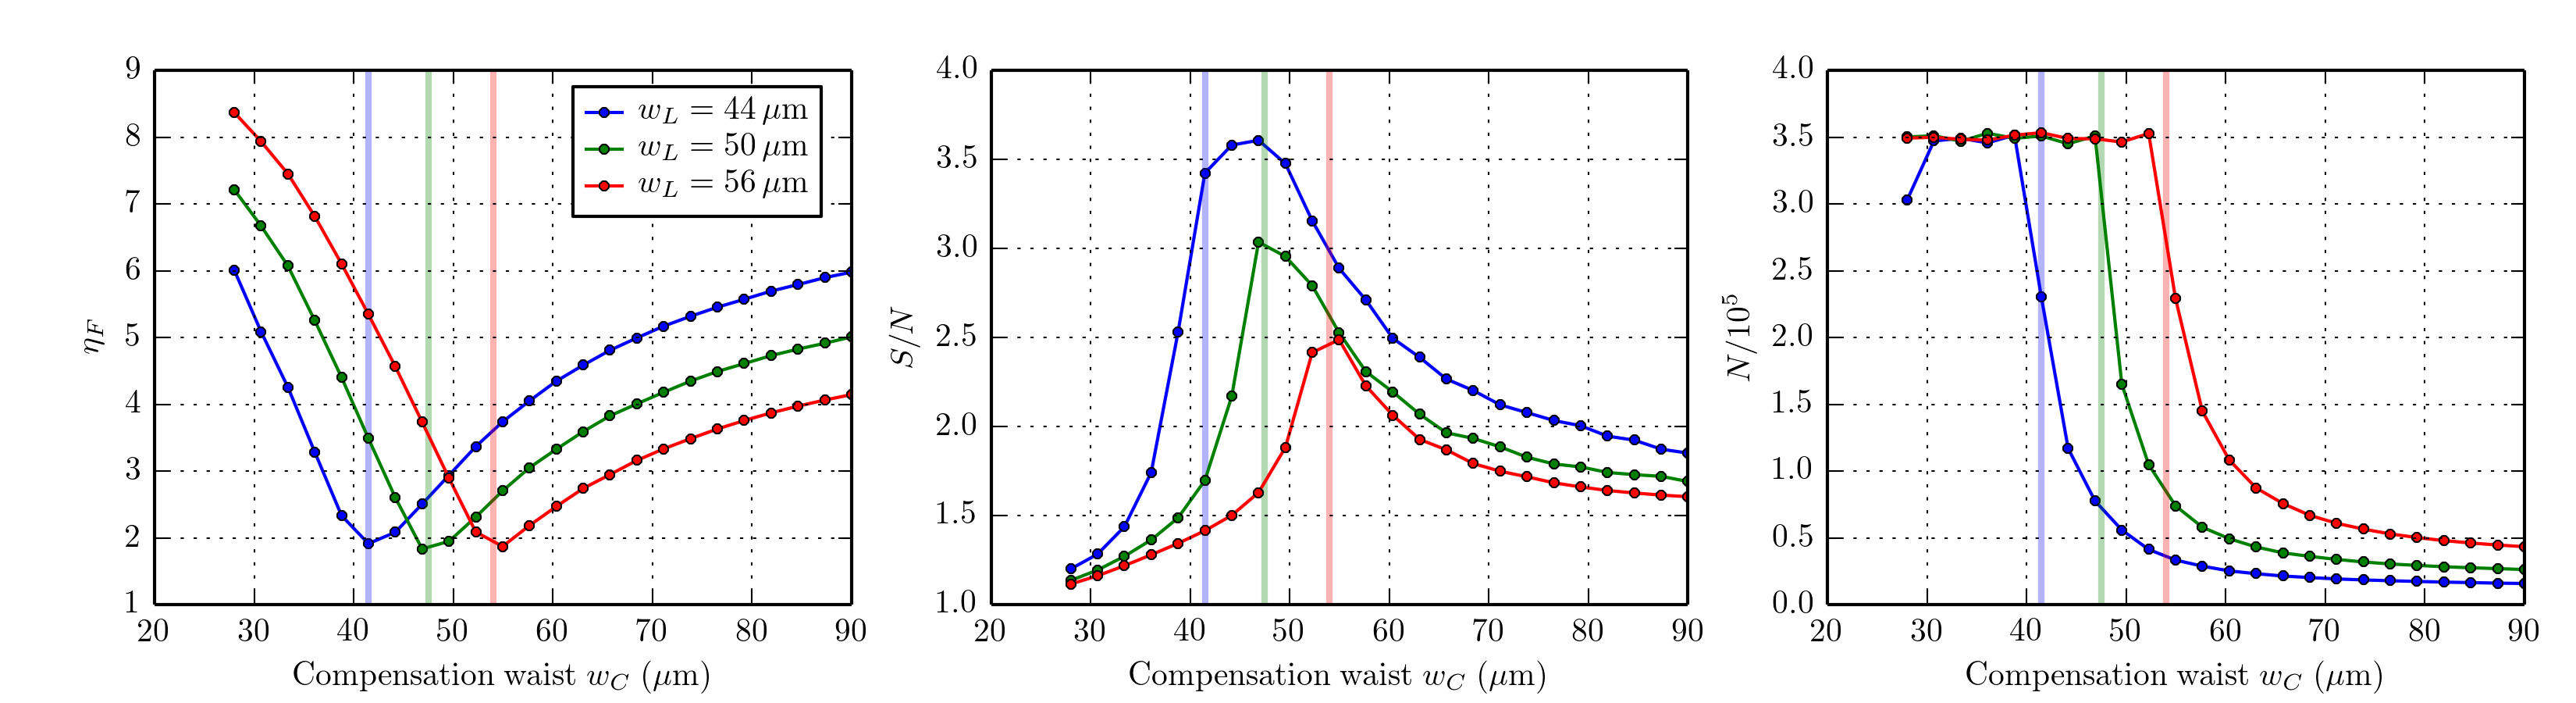
\includegraphics[width=\textwidth]{figures/etaF-wIRwGR-lines.png} \caption{
$\eta_{F}$, $S/N$, and $N$ as a function of $w_{C}$ for various values of $w_{L}$.  }
\label{fig:etaF-wIRwGR-lines}
\end{figure}
Given this observation,  we now set $w_{L}=w_{C}$ and vary both together  to see
if it is favorable to make smaller or larger beam waists.  This is shown in
Fig.~\ref{fig:etaF-wIR=wGR}.  The main observations are:
\begin{itemize}
\item  For beam waists up to $\approx68\,\mu$m one can keep getting lower
$\eta_{F}$ by making the beam waists larger.  This trend would continue if we
had an unlimited number of atoms, however beyond $\approx68\,\mu$m the number
of atoms required to fill the trap goes above our cap of 350,000 atoms.  
\item
For larger beam waists the entropy capacity is always lower, so the choice of
beam waist will be a compromise between $\eta_{F}$ and the entropy capacity. 
\end{itemize} 
\begin{figure}
    \centering 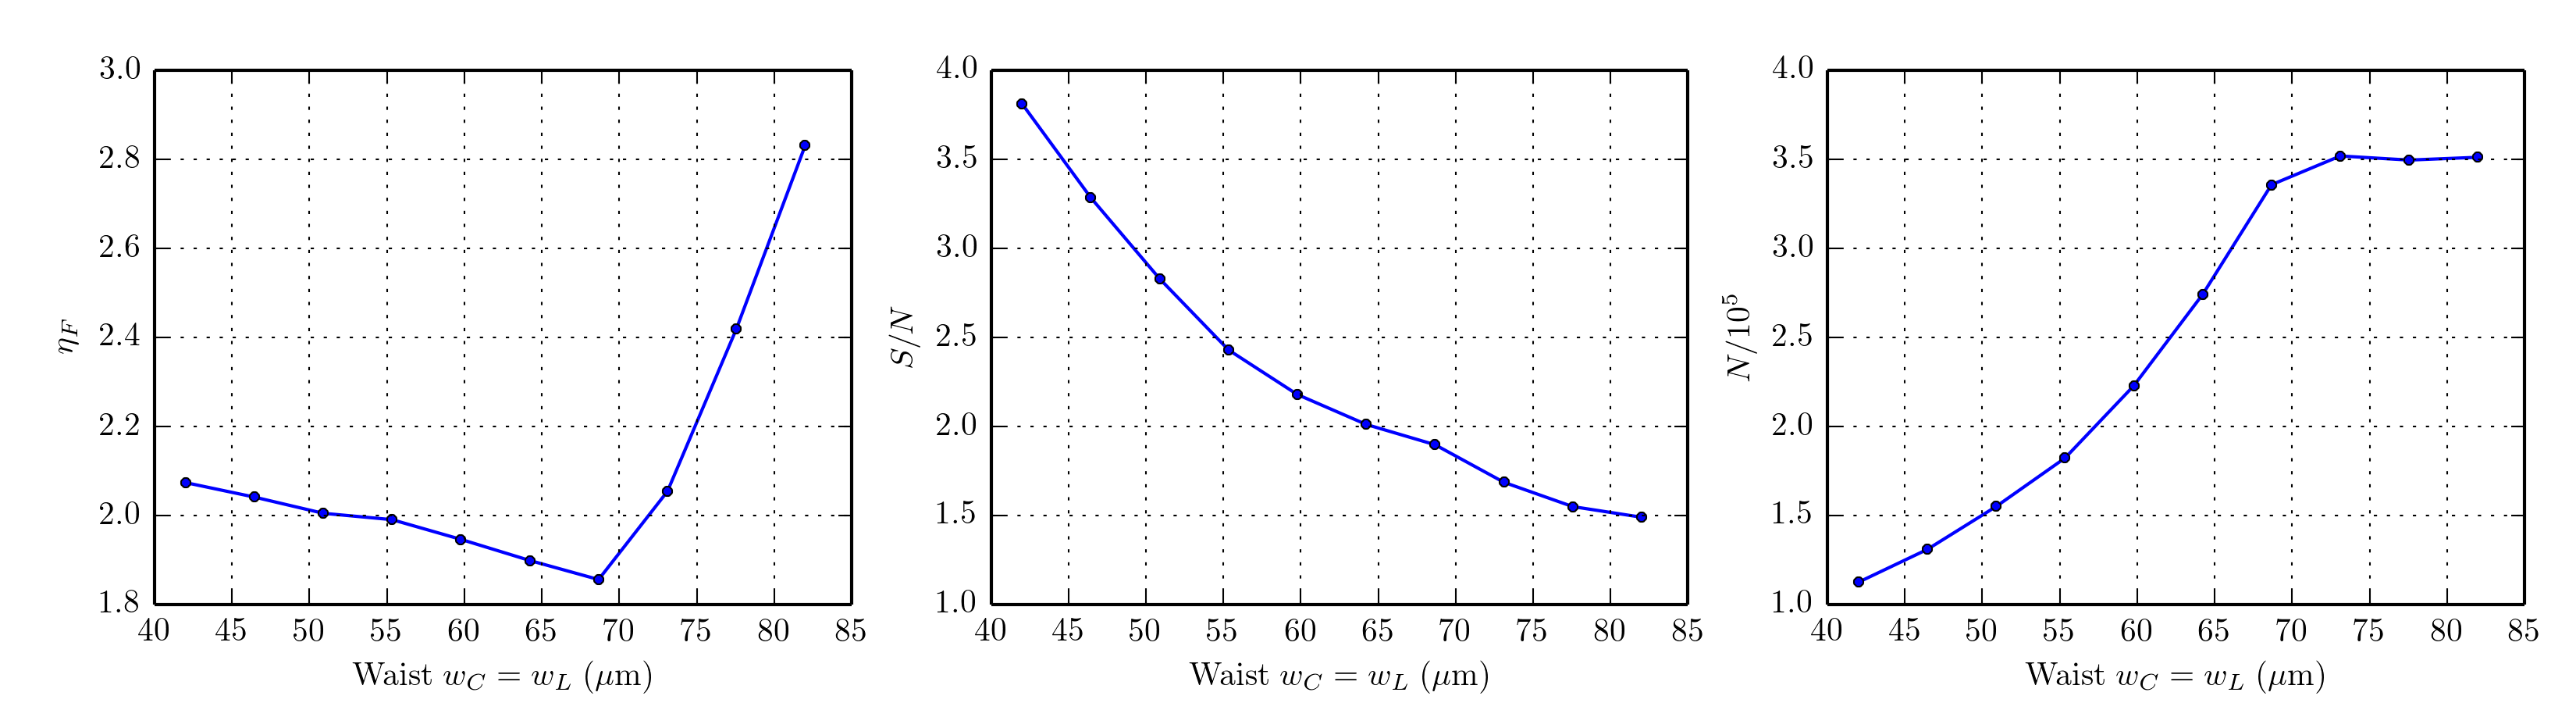
\includegraphics[width=\textwidth]{figures/etaF-wIR=wGR.png}
\caption{ $\eta_{F}$ and $S/N$ as a function of beam waist for $w_{L}=w_{C}$.
Results are shown for various atom numbers.  }
\label{fig:etaF-wIR=wGR}
\end{figure}

%In my opinion, the choice of beam waist should exploit the number of atoms that
%we have at our disposal


The results shown in Figs.~\ref{fig:etaF-wIR=wGR},~\ref{fig:etaF-wIRwGR-lines}
show that it is desirable to have equal lattice and compensation beam waists.
The choice of their value is a compromise between the achievable $\eta_{F}$ and
the entropy capacity, given by $S/N$.   Another important experimental
constraint is the available of power at the lattice and compensation
wavelengths, which is a bigger issue for larger beam waists.  In that case
larger power is necessary to achieve the required potential depths.   The
compensation power needed to compensate a 7\,$E_{R}$ lattice and the lattice
power needed to make a 40\,$E_{R}$ deep lattice\footnote{If we want to freeze
out tunneling in the lattice we required depths as large as 40\,$E_{R}$ where
the tunneling rate goes down to 3\,Hz.  We currently ``lock'' the lattice at
20\,$E_{R}$ for our Bragg scattering measurements.  At 20\,$E_{R}$ the
tunneling rate is 72\,Hz. This is good enough for Bragg scattering, but not
good enough for measurements that take longer, such as associating through the
narrow Feshbach resonance to measure double occupancies. } are shown in
Fig.~\ref{fig:green-power-wIR=wGR}.   With this in mind and our available
powers we can safely realize any choice of beam waists below $65\,\mu$m. 
\begin{figure}
    \centering
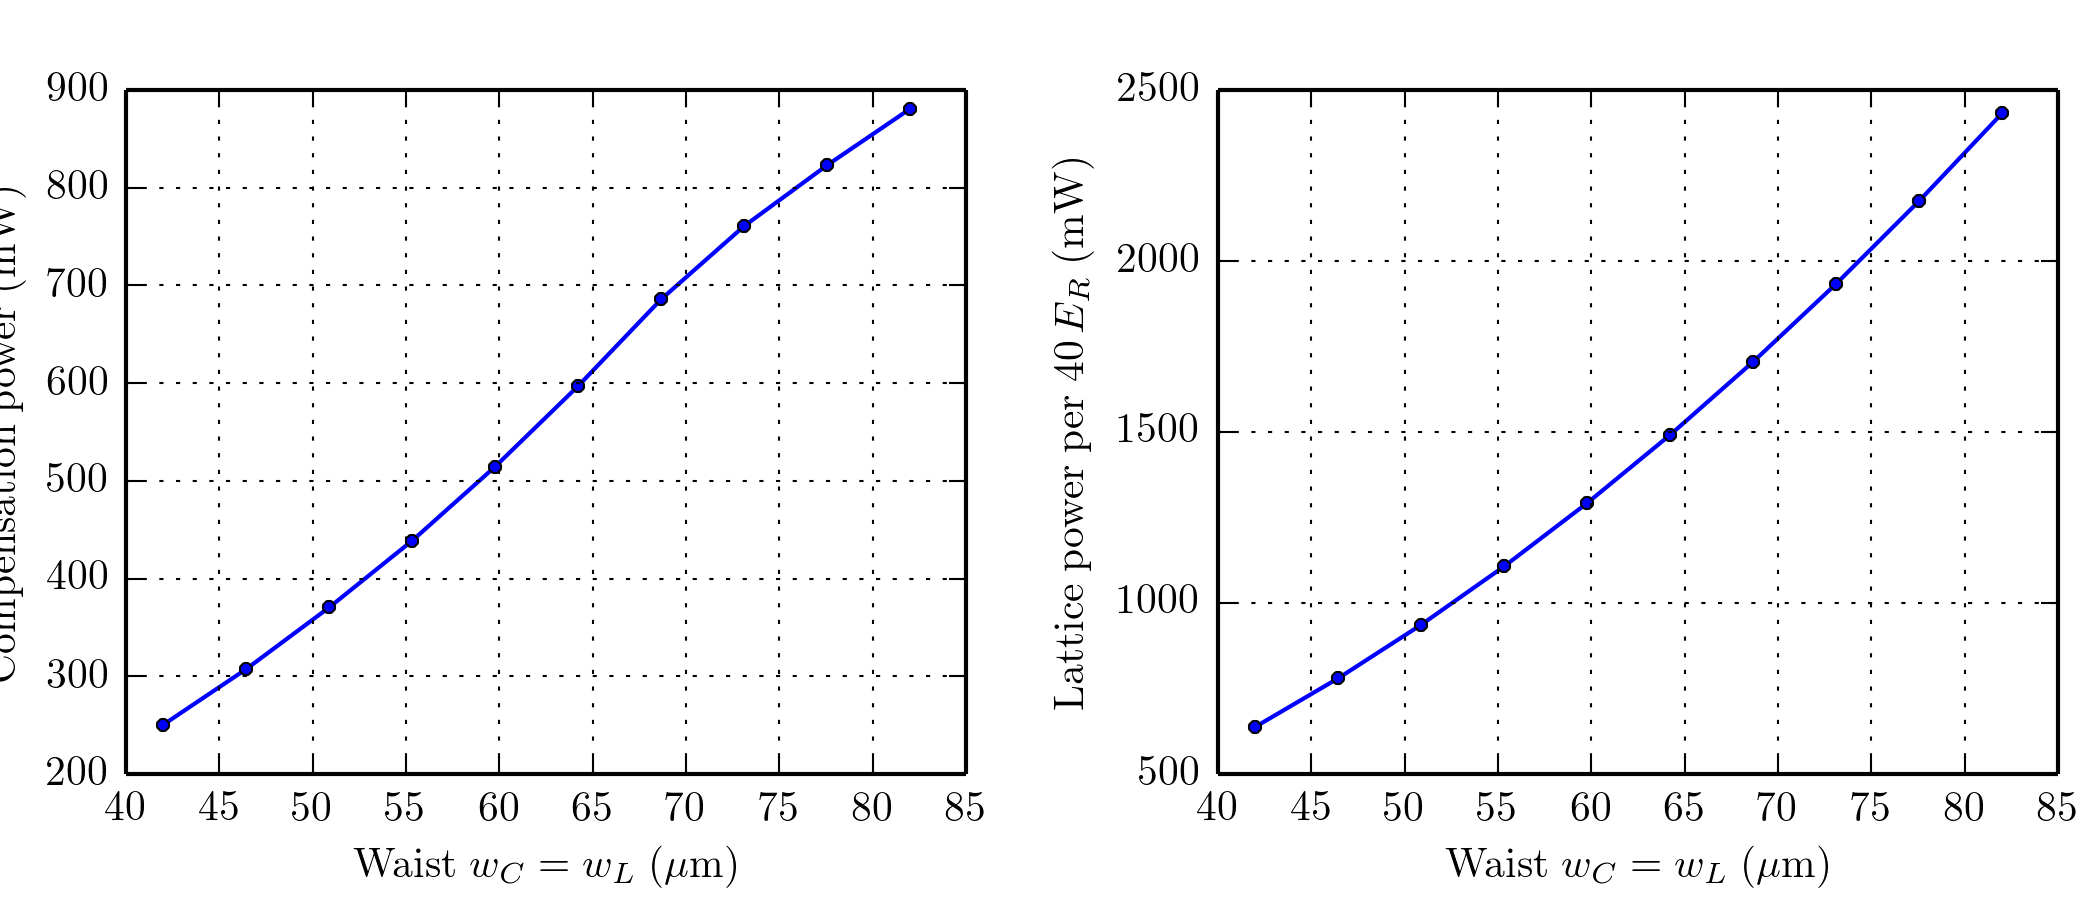
\includegraphics[width=0.7\textwidth]{figures/green-power-wIR=wGR.png}
\caption{ Compensation power required to compensate a 7\,$E_{R}$ lattice and
lattice powered required to achieve a 40\,$E_{R}$ lattice depth.  }
\label{fig:green-power-wIR=wGR}
\end{figure}

To fully exploit the atom number that we can produce in our experiment our
opinion is to go to the larger lattice beam waists,  so we recommend values of
$w_{L}=w_{C}=65\,\mu$m.   These proposed parameters  would change the
evaporation factor and entropy capacity and number capacity of our setup
according to the following table:
\begin{center}
\begin{tabular}{ c|c|c|c|c|c}
   &  $w_{L}\,(\mu\mathrm{m})$ & $w_{C}\,(\mu\mathrm{m})$ 
   & $\eta_{F}$  & $\xi_{\text{evap}}$ &  $S/N$  \\ \hline 
 Current setup &  47 & 40  &  2.95 & $3.4\times 10^{-10}$  &   1.94  \\ 
 Proposed change & 65 & 65  &  1.52 & $1.36\times 10^{-5}$  &   1.99  \\
\end{tabular}
\end{center}
We see that for the optimal beam waist ratio a value of
$\xi_{\text{evap}}\sim10^{-5}$ may be reached that could lead to reasonable
rates of evaporation in the lattice.  A comparison of our current setup and
this proposed scenario is shown in Fig.~\ref{fig:etaF-before-after}. 
\begin{figure}
        \centering
        \begin{subfigure}[t]{0.45\textwidth}
		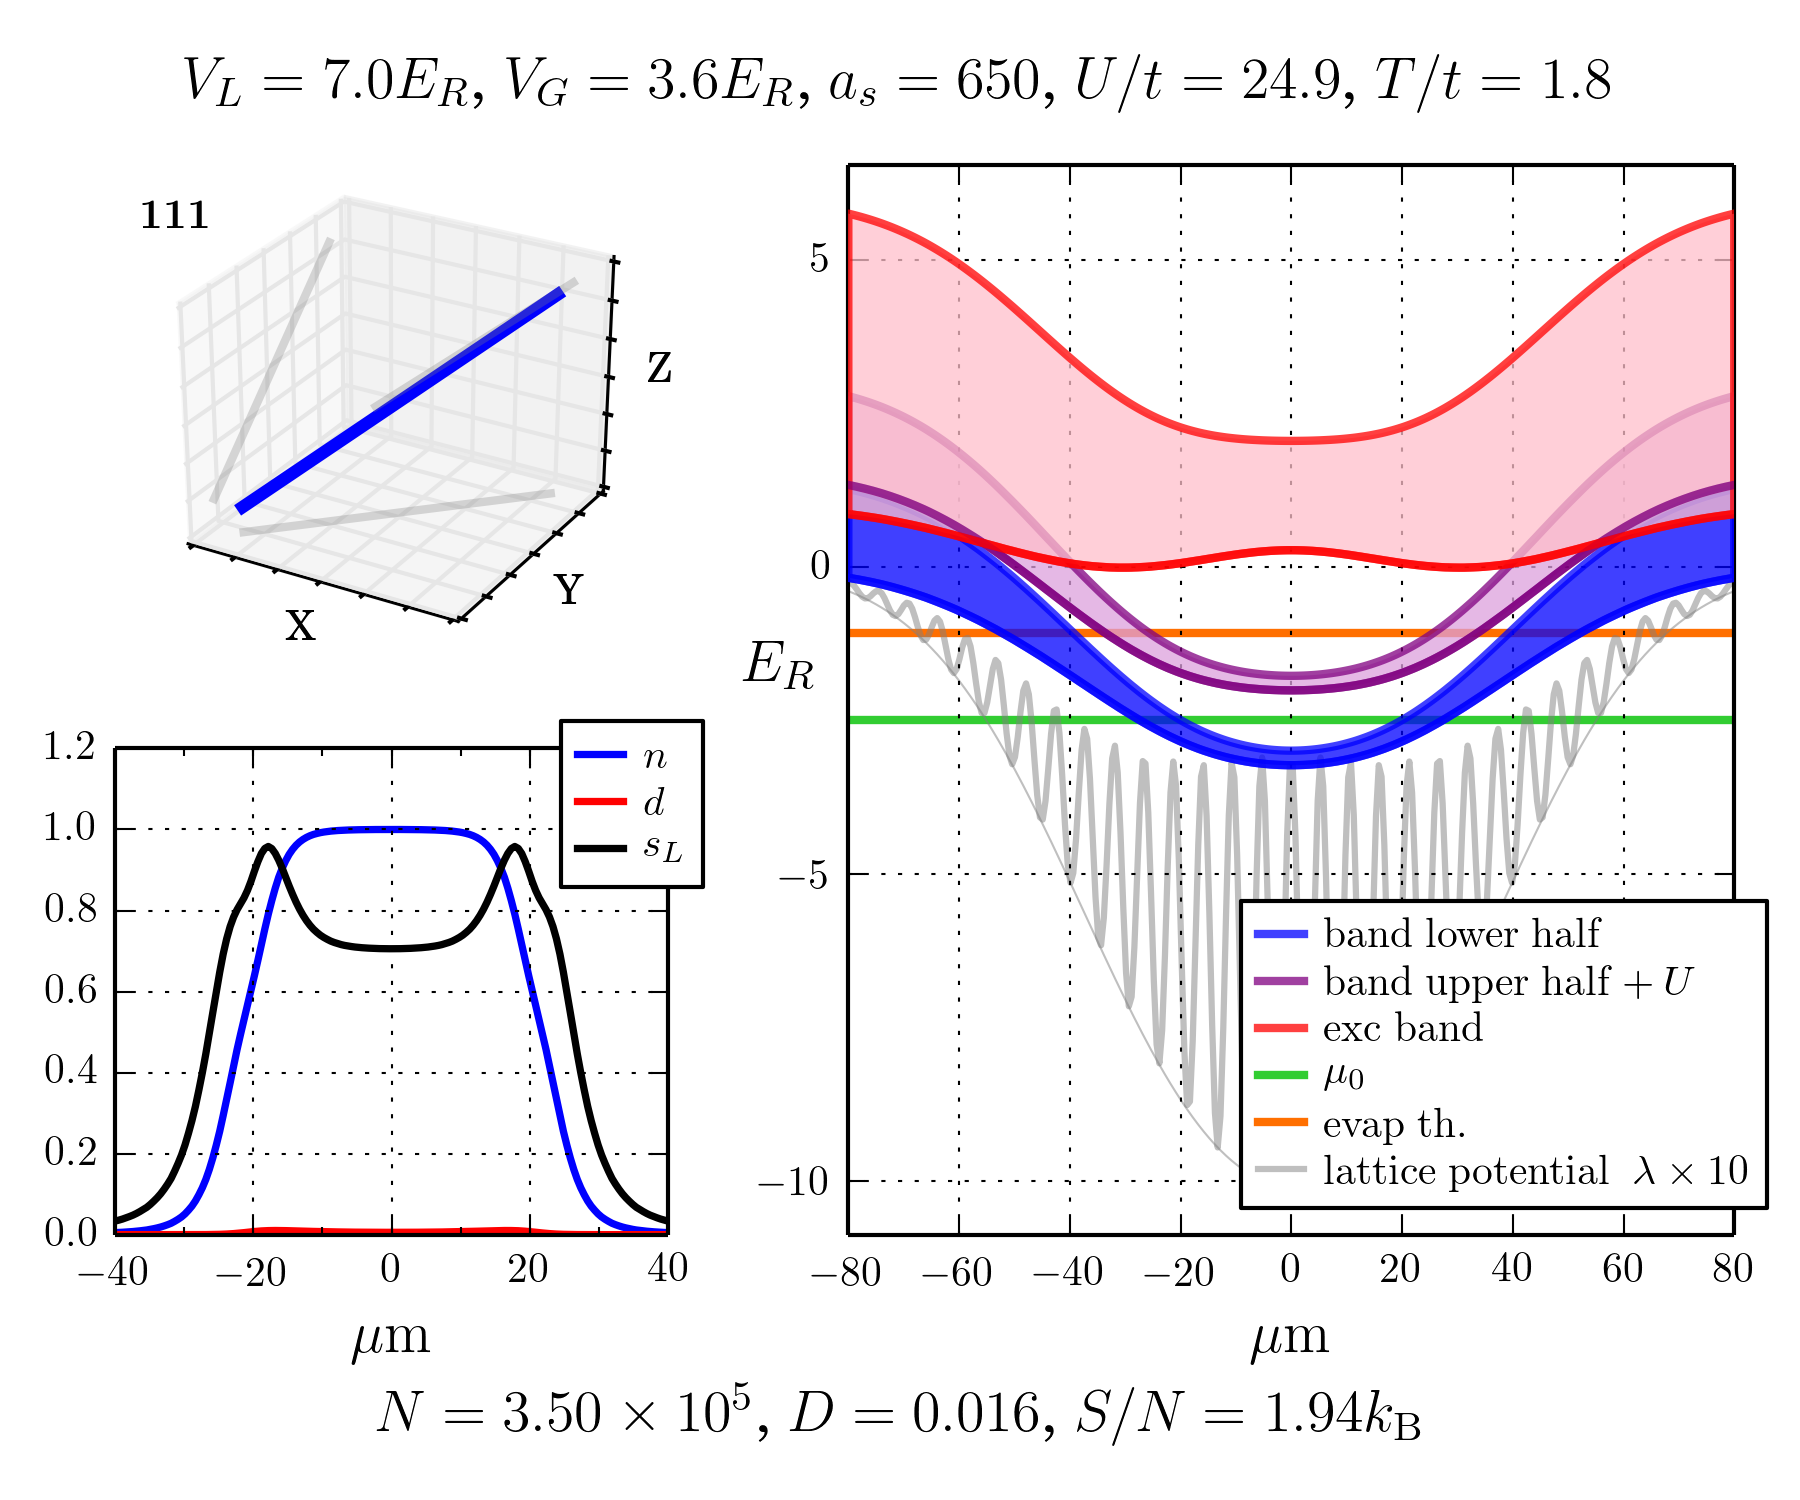
\includegraphics[width=\textwidth]{figures/ir47-gr40_7Er-comp3p642.png}
\caption{ $w_{L} = 47\,\mu$m and $w_{C}=40\,\mu$m.  Compensation is chosen so
that unit filling is achieved at the center for an atom number of 350,000. }
        \end{subfigure}
        ~ %add desired spacing between images, e. g. ~, \quad, \qquad etc.
          %(or a blank line to force the subfigure onto a new line)
        \begin{subfigure}[t]{0.45\textwidth}
		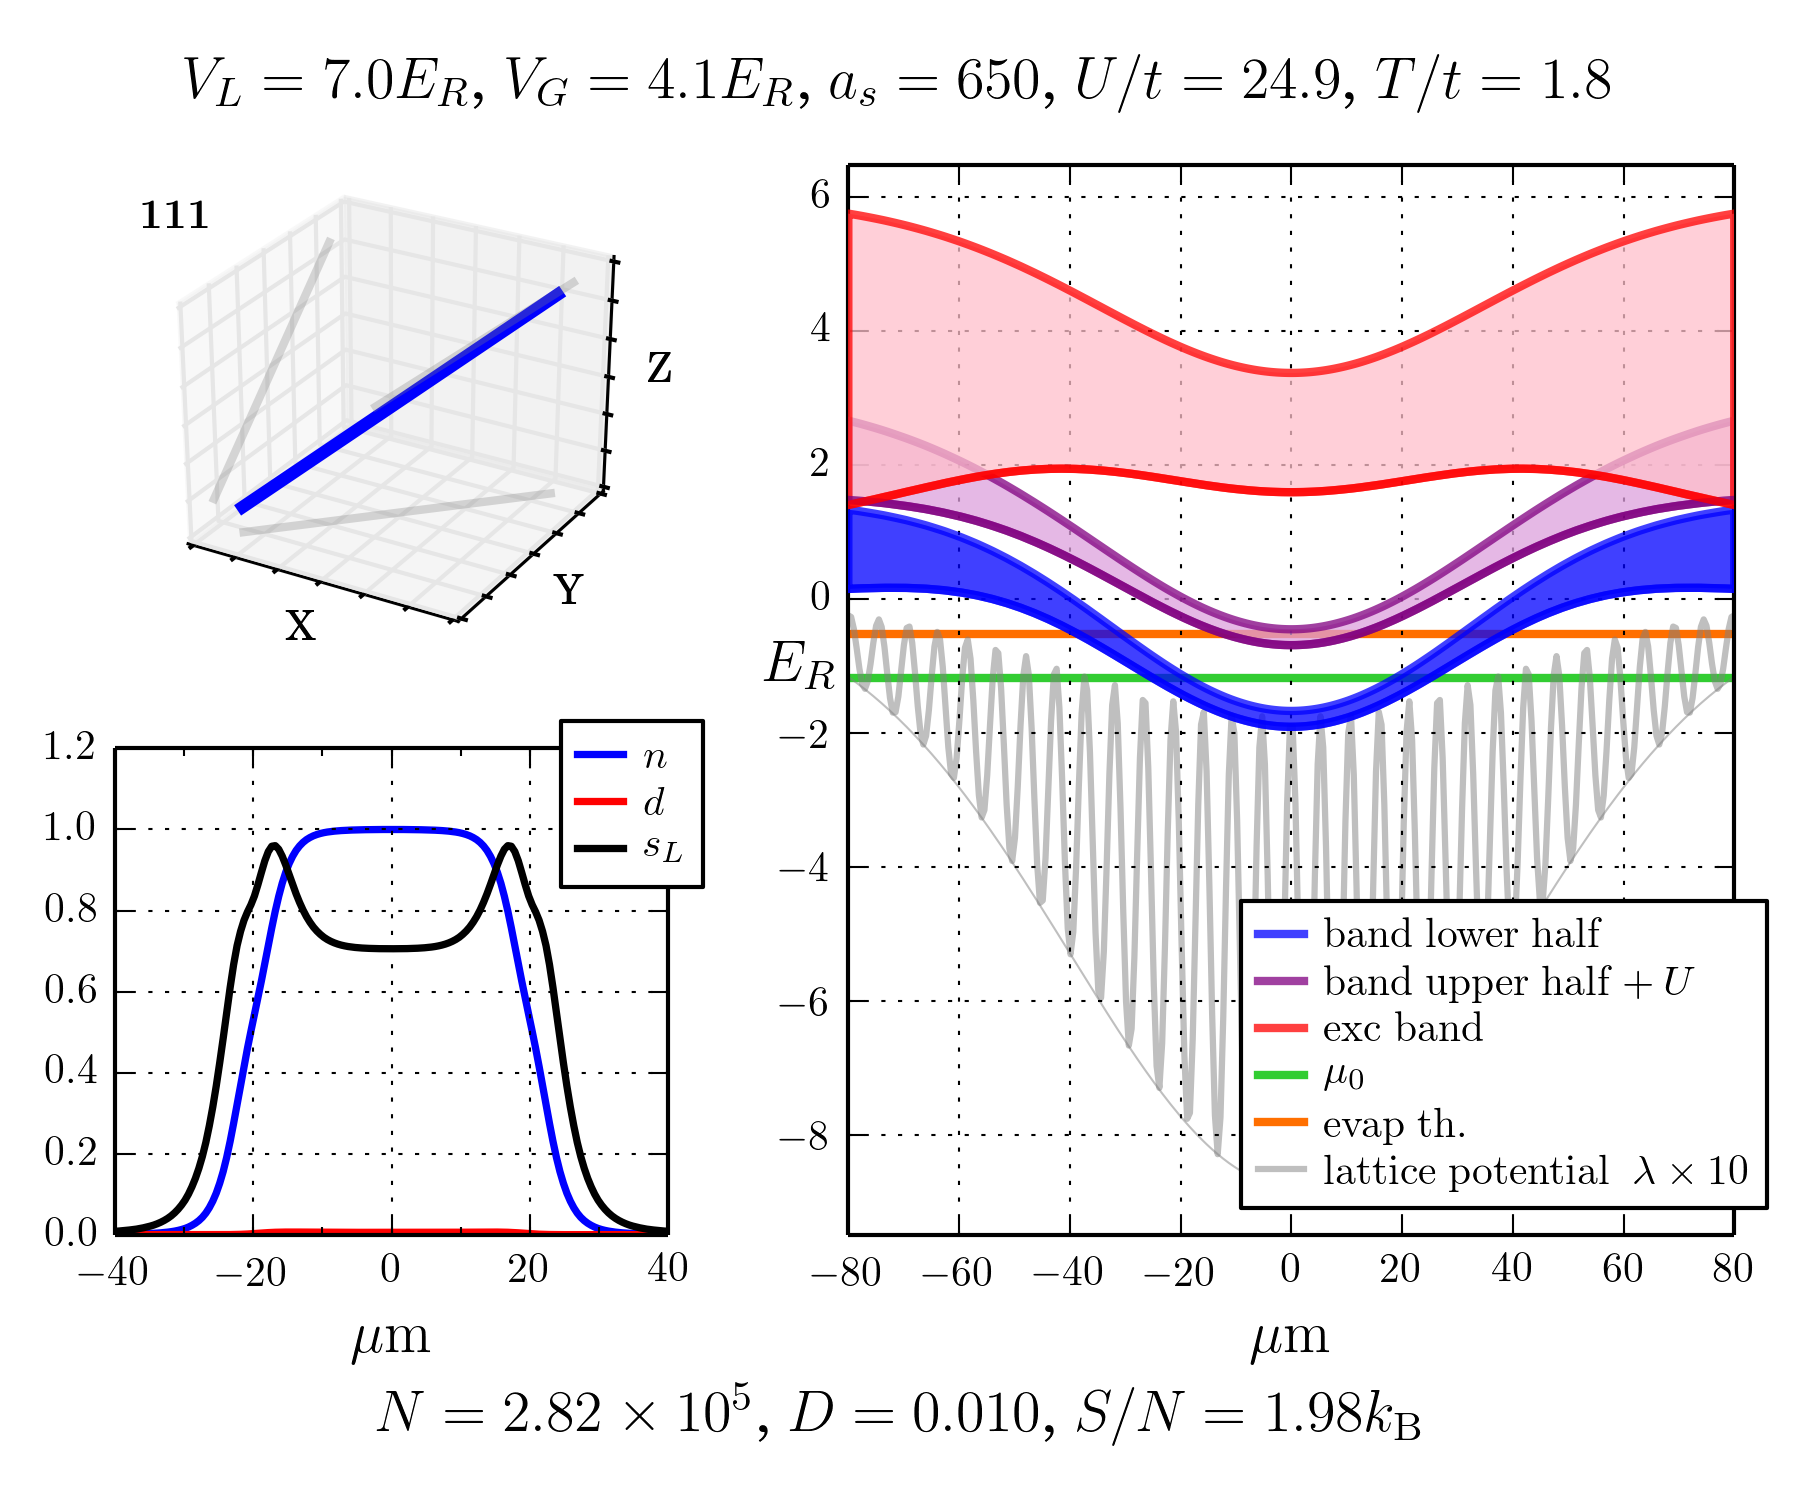
\includegraphics[width=\textwidth]{figures/ir65-gr65_7Er-comp4p08.png}
\caption{ $w_{L} = 65\,\mu$m and $w_{C}=65\,\mu$m.  Atom number maxes out at 284,000 atoms. }
        \end{subfigure}%
	\caption{Full trap profiles of band structure and thermodynamic
quantities for our current setup and the proposed setup with equal beam waists.} 
\label{fig:etaF-before-after}
\end{figure}

 



 
\section{ Conclusions }


\bibliographystyle{osa}
\bibliography{latt_evap}

\end{document}




